\chapter{Proof of Concepts}%
\label{ch:proof-of-concepts}

\section{Azure Data Factory (ADF)}

\subsection{Opzet van resources}

Door in Microsoft Azure naar Data Factories te navigeren kan een nieuwe data factory aangemaakt worden.

\begin{figure}[H]
    \centering
    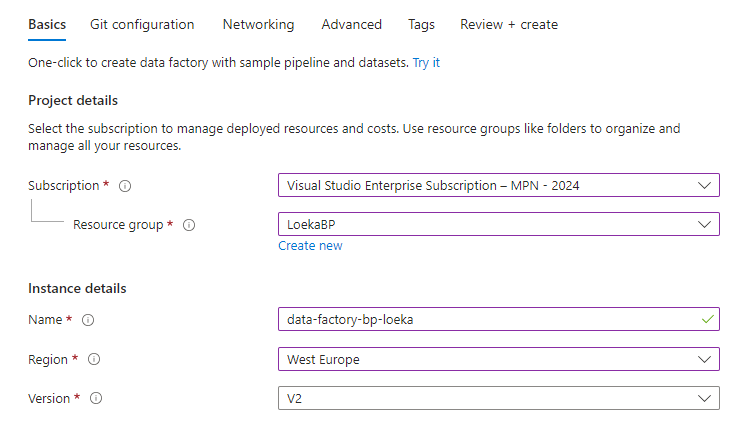
\includegraphics[width=1\textwidth]{./graphics/adf/initial_create.png}
    \caption{Aanmaken van Azure Data Factory}
\end{figure}

% Resource group en subscription in literatuurstudie
Bij het aanmaken van een data factory moet er een subscription en resource group gekozen worden. Er kan een nieuwe resource group aangemaakt worden of een reeds bestaande gekozen worden. Daarnaast moet er een naam, gewenste regio en versie voor Data Factory gekozen worden. Git configuratie komt later aan bod. Wanneer de resource is aangemaakt kan Azure Data Factory opgestart worden.

\subsection{Collaboration en source control}
\label{sec:adf-git}

Binnen Azure Data Factory kan er op 2 manieren samen gewerkt worden. 

\subsubsection{Roles en permissions}

\begin{figure}[H]
    \centering
    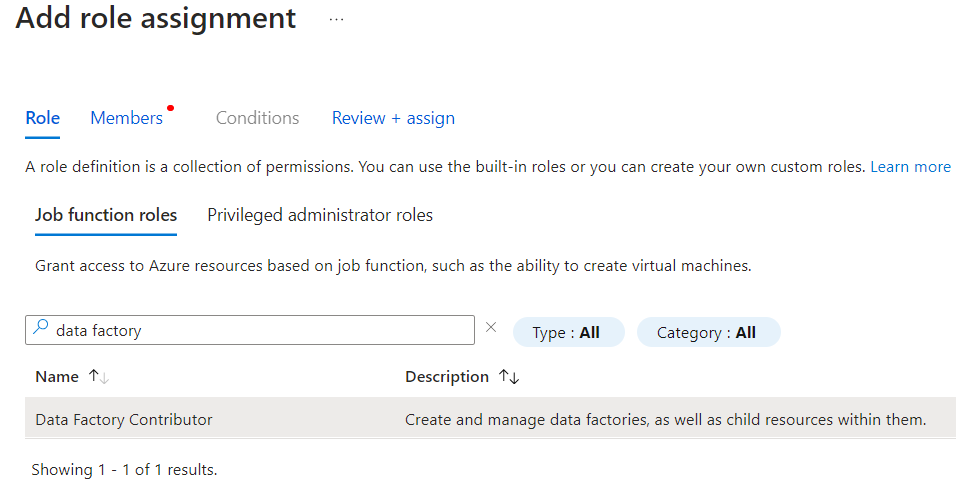
\includegraphics[width=1\textwidth]{./graphics/adf/adf_contributor.png}
    \caption{Toewijzen van Data Factory Contributor Role}
\end{figure}

Door de bij de resource group van de data factory de Data Factory Contributor role toe te wijzen kan men toegang geven tot volgende zaken:
\begin{itemize}
    \item Het aanmaken, wijzigen en verwijderen van data factories en child resources
    \item Deployment van Resource Manager templates
    \item Het managen van App Insight alerts voor Data Factory
    \item Het aanmaken van support tickets
\end{itemize}

\subsubsection{Source control}

Azure Data Factory laat het toe om een Git repository te configureren via Azure Repos of GitHub. We kiezen hier voor Azure DevOps doordat er binnen Net IT hier mee gewerkt word.

%\begin{figure}[H]
%    \centering
%    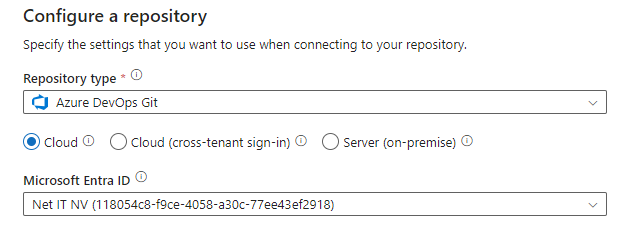
\includegraphics[width=0.8\textwidth]{./graphics/adf/setup_repository_2_specific.png}
%    \caption{Configuratie van Git in Azure Data Factory}
%\end{figure}

%We kiezen voor Azure DevOps doordat er binnen Net IT hiermee gewerkt wordt.

\begin{figure}[H]
    \centering
    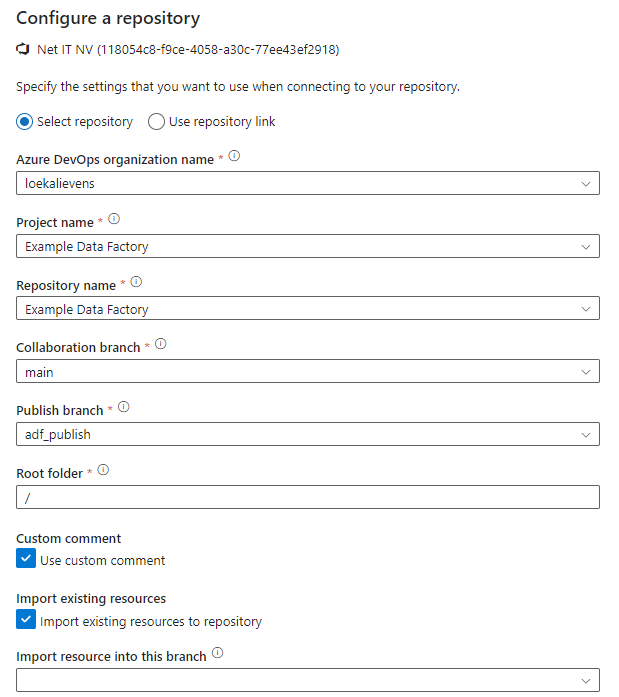
\includegraphics[width=0.8\textwidth]{./graphics/adf/setup_repository_3_specific.png}
    \caption{Configuratie van Azure DevOps in Azure Data Factory}
\end{figure}

De collaboration branch is de enigste branch waarbij de publish knop zichtbaar zal zijn. Door te werken met feature branches en hiermee pull requests te maken op de collaboration branch kan er dus samen gewerkt worden. De publish branch is de branch waar alle ARM templates van de gepubliceerde factory opgeslaan worden.

% In literatuurstudie meer uitleg over de collaboration branch

\subsection{IDE integratie}

Met behulp van de ``Azure Data Factory tools for Visual Studio'' extensie kunnen data pipelines ontwikkeld worden in Visual Studio. Ook nu kunnen deze visueel ontwikkeld worden of kunnen de Azure Data Factory JSON bestanden met behulp van IntelliSense en schema-validatie bewerkt worden.

\subsection{Infrastructure as code (IaC)}

Azure Data Factory maakt gebruik van Azure Resource Manager (ARM) templates voor het opslaan van configuratie van verschillende ADF entiteiten zoals bijvoorbeeld pipelines, datasets, dataflows, enzovoort. Hiermee kan een data factory verplaatst worden naar een andere omgeving. Dit kan automatisch met behulp van Azure Pipelines of handmatig door een ARM template te uploaden via de Data Factory UX. Zoals te zien in sectie~\ref{sec:adf-git} is Git integreerbaar in Azure Data Factory. Hier in worden de ARM templates opgeslaan op de publish branch. Met behulp van Continuous Integration (CI) en Continuous Deployment (CD) via DevOps-pipelines kunnen aanpassingen die gebeuren op een bepaalde Git-repository dan automatisch gevalideert, getest en uitgerold worden naar een doelomgeving.

\subsection{Ophalen van data uit Azure Data Lake}

Het ophalen van data uit Data Lake in Data Flow gebeurd steeds op dezelfde manier. 

\begin{figure}[H]
    \centering
    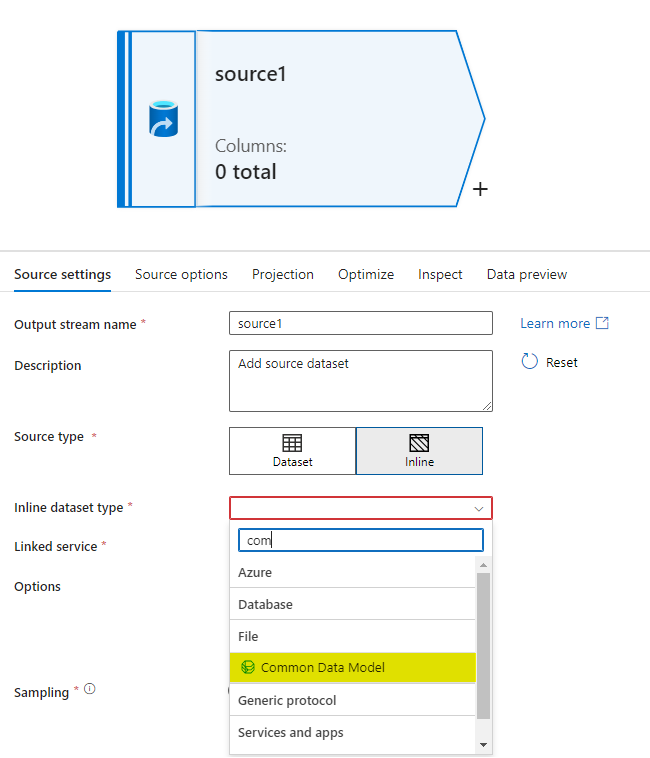
\includegraphics[width=0.8\textwidth]{./graphics/adf/source_table_1_specific.png}
    \caption{Configuratie van source transformation}
\end{figure}

Als source type wordt er steeds gekozen voor ``inline''. Dit doordat we slechts werken met één enkele dataflow en geen gedeelde datasets nodig hebben. Als inline data set type kiezen we voor Common Data Model.

\begin{figure}[H]
    \centering
    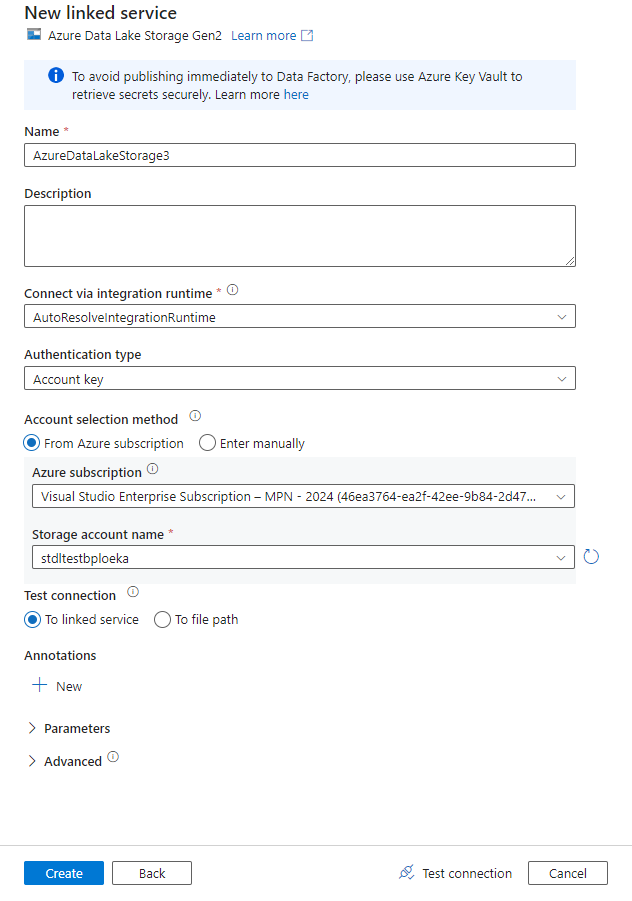
\includegraphics[width=0.8\textwidth]{./graphics/adf/source_table_3_specific}
    \caption{Configuratie van Linked Service}
    \label{fig:linked-service}
\end{figure}

Er zal éénmalig een Linked Service aangemaakt moeten worden. Hierbij kiezen we voor Azure Data Lake Storage Gen2. We kunnen makkelijk gaan koppelen met de juiste data lake door een Azure Subscription en Storage account name aan te duiden. Door op ``Test connection'' te klikken kunnen we kijken of de connectie met data lake is gelukt. Door op ``Create'' te klikken hebben we nu een Linked Service die steeds bij elke Source gebruikt kan worden.

\textbf{Let op:} Doordat Git geen secrets opslaat is het aanbevolen om gebruik te maken van Azure Key Vault voor het opslaan van connection strings of passwords.

\begin{figure}[H]
    \centering
    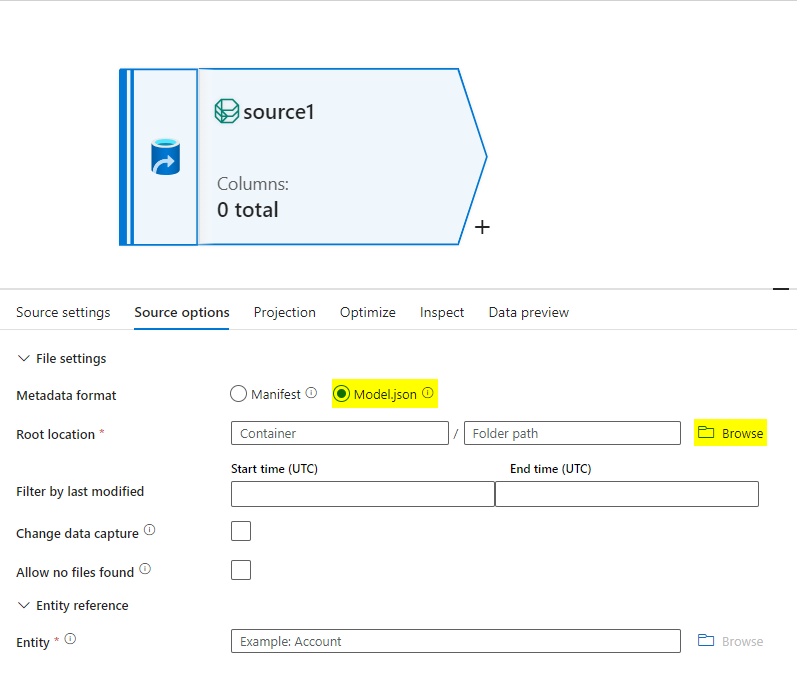
\includegraphics[width=0.9\textwidth]{./graphics/adf/source_table_4_specific.png}
    \caption{Configuratie van source options}
\end{figure}

Onder ``Source options'' wordt ``Model.json'' aangeduid. Door hierna op ``Browse'' te klikken kan er aangeduid worden waar het Model.json bestand te vinden is in Data Lake. Dit JSON bestand beschrijft hoe de data in Data Lake er uit ziet.

\begin{figure}[H]
    \centering
    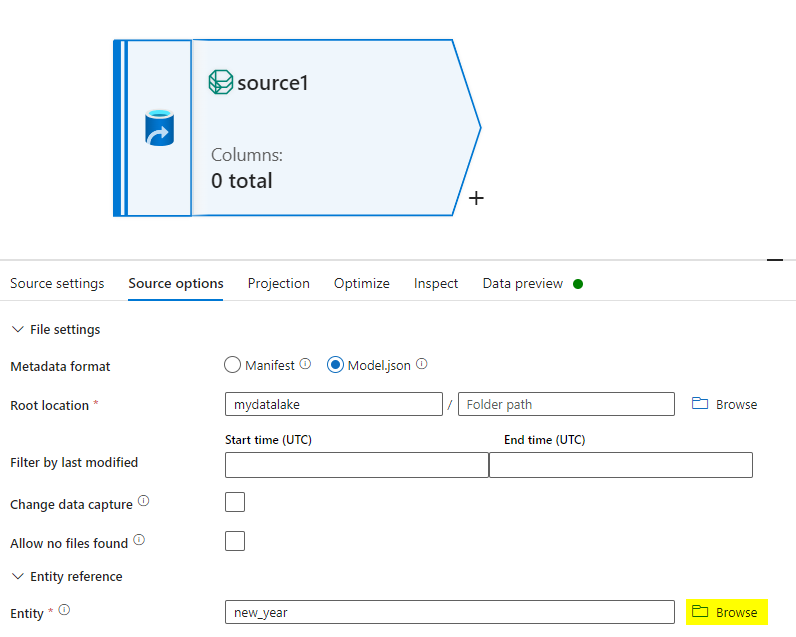
\includegraphics[width=0.9\textwidth]{./graphics/adf/source_table_5_specific.png}
    \caption{Configuratie van source options}
\end{figure}

De gewenste entiteit kan nu geselecteerd worden door op ``Browse'' naast ``Entity'' te klikken. Let op: hier voor zal Data flow debug aan moeten staan.

\begin{figure}[H]
    \centering
    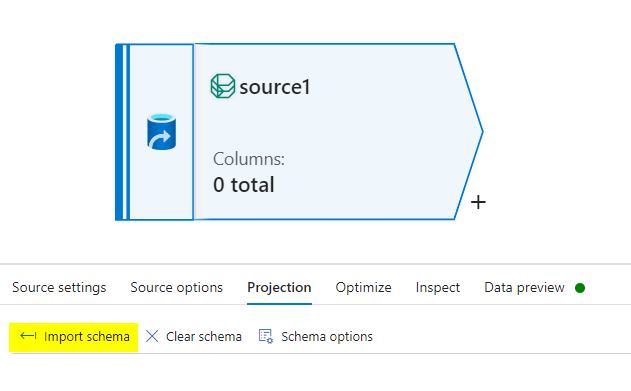
\includegraphics[width=0.8\textwidth]{./graphics/adf/source_table_6_specific.png}
    \caption{Importeren van schema voor data flow source}
\end{figure}

Onder ``Projection'' kan er nu op ``Import schema'' geklikt worden om de verschillende kolommen met bijhorende types op te halen.

\begin{figure}[H]
    \centering
    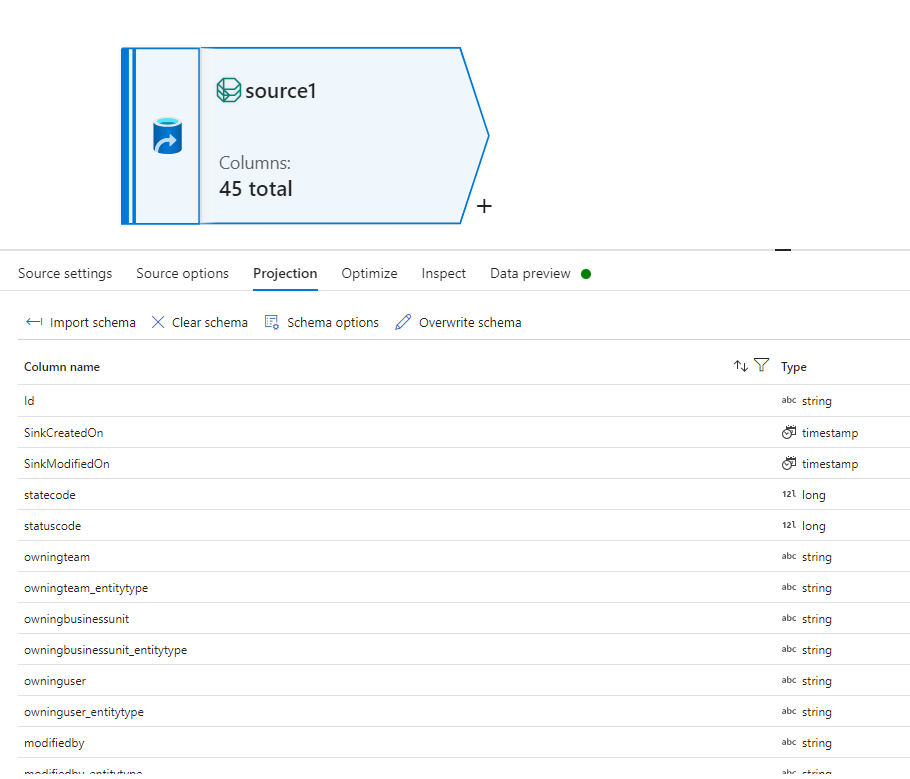
\includegraphics[width=0.9\textwidth]{./graphics/adf/source_table_7_specific.png}
    \caption{Voorbeeld geïmporteerd schema van data flow source}
\end{figure}

De foto hierboven toont een voorbeeld van een geïmporteerd schema.

\begin{figure}[H]
    \centering
    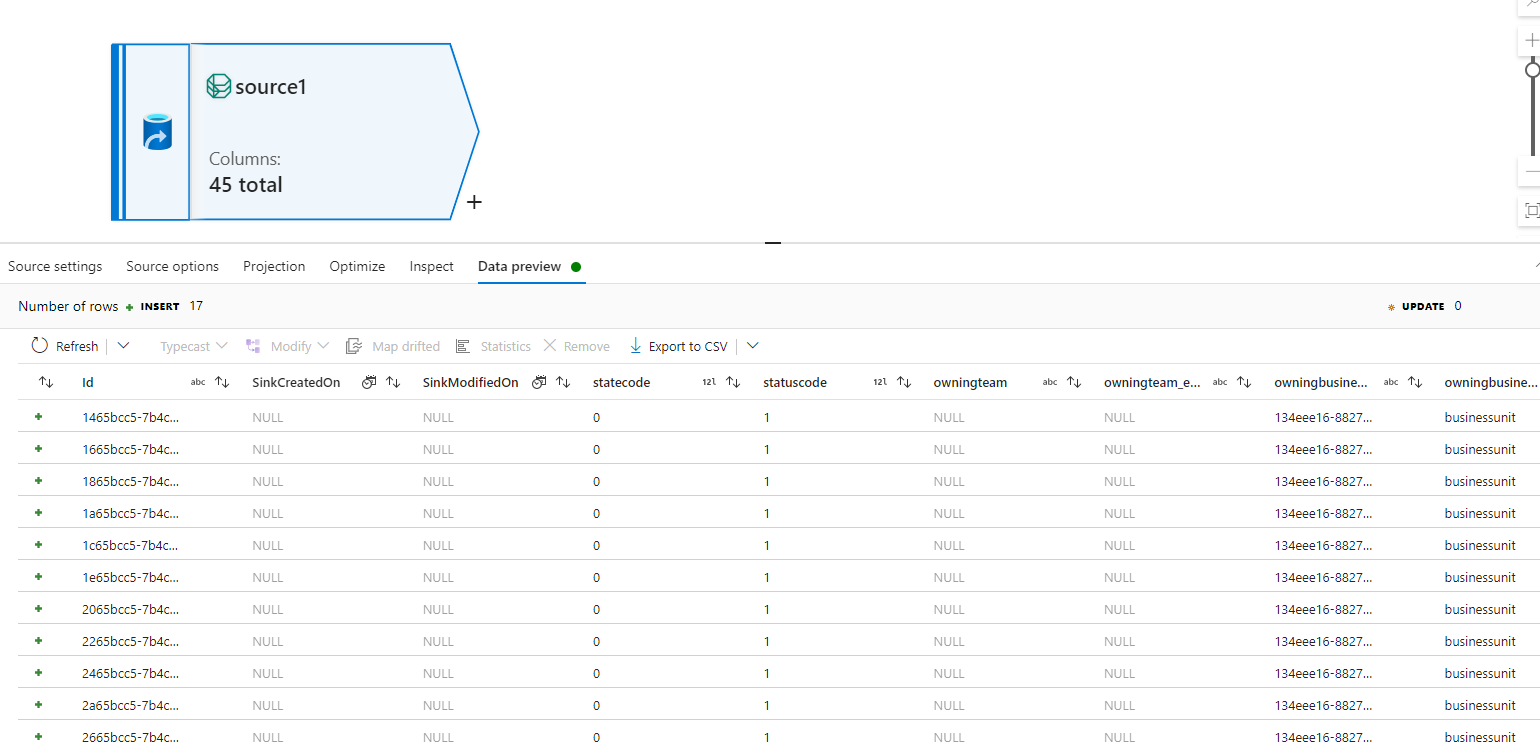
\includegraphics[width=1\textwidth]{./graphics/adf/source_table_8_specific.png}
    \caption{Data preview in data flow}
    \label{fig:data-preview}
\end{figure}

Door naar ``Data preview'' te navigeren kan er een preview bekeken worden van de data uit de gekozen tabel. Dit kan bij elke transformatie die er in data flow gebeurd. Ook hier voor moet Data flow debug aan staan.

\subsection{Mogelijkheid tot debuggen}

Zoals te zien op Figuur~\ref{fig:data-preview} kan er per transformatie een data preview getoond worden. Dit is een tabel die toont hoe de data na de transformatie er uit ziet. Belangrijk om hierbij te weten is dat ``Data flow debug'' aan zal moeten staan en er dus ook kosten in rekening gebracht zullen worden. Per tabel zal er standaard ook slechts 1000 rijen opgehaald worden. Voor kleine pipelines zal dit dus geen probleem zijn maar voor deze pipeline moest deze limiet verhoogd worden. Daarnaast kan dit soms heel traag worden wanneer de transformaties complex worden.

\pagebreak 

\subsection{Belangrijkste transformaties}

\subsubsection{Determinatie van welke groepen de premie in hun bestand krijgen}

\begin{figure}[H]
    \centering
    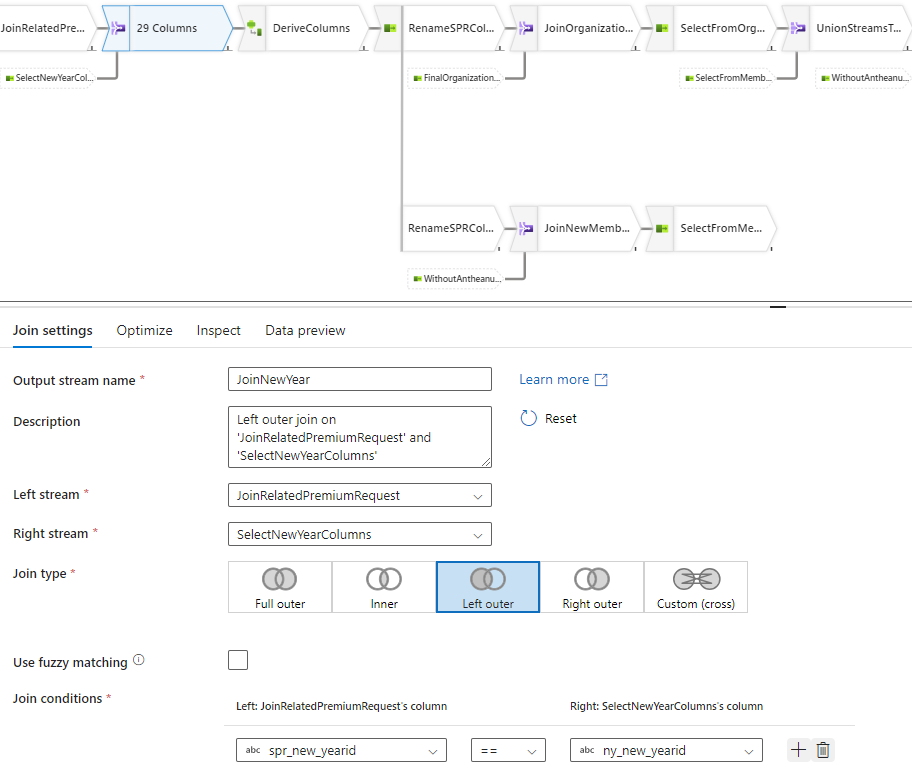
\includegraphics[width=0.9\textwidth]{./graphics/adf/bepalen_groep_1.png}
    \caption{Join van de tabel ``new\_year'' op de tabel ``new\_syndicalpremiumrequest''}
\end{figure}

De tabel ``new\_syndicalpremiumrequest'' heeft een kolom ``spr\_new\_yearid''. Om te gaan bepalen wat het referentiejaar van deze premie is zal dus de tabel ``new\_year'' op de tabel ``new\_syndicalpremiumrequest'' gejoind moeten worden aan de hand van dit id.


\begin{figure}[H]
    \centering
    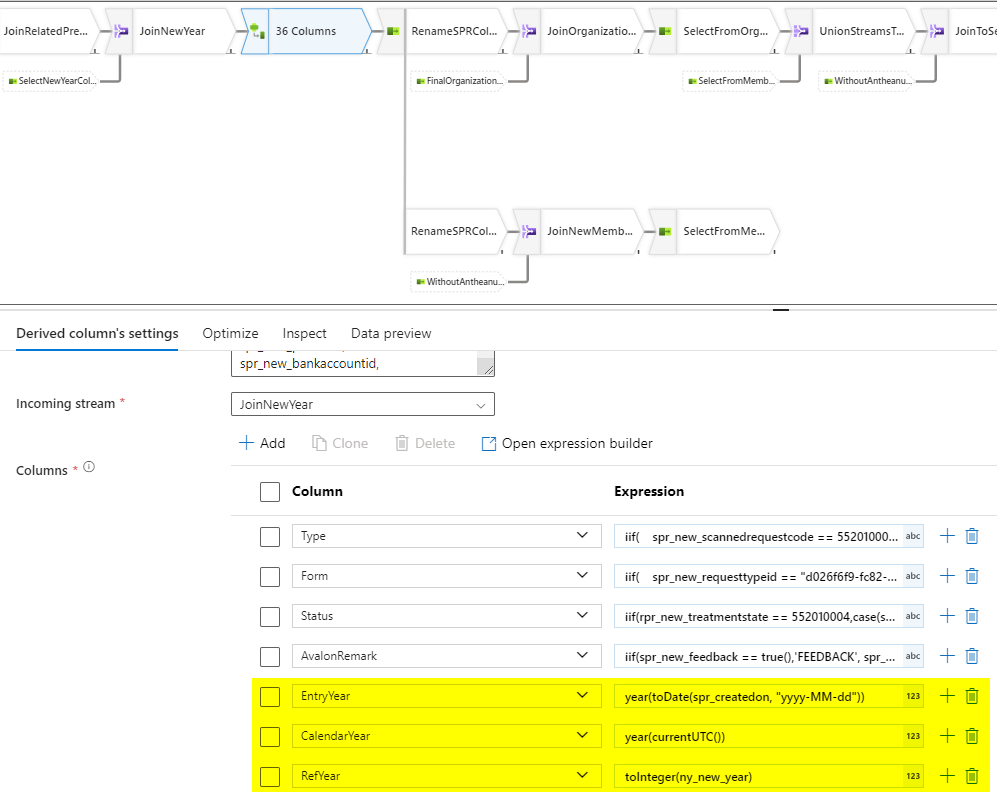
\includegraphics[width=1\textwidth]{./graphics/adf/bepalen_groep_2.png}
    \caption{Derive ``EntryYear'', ``CalendarYear'' en ``RefYear'' op de tabel ``new\_syndicalpremiumrequest''}
\end{figure}

Voor het bepalen van de groepen hebben we 3 nieuwe kolommen nodig. Als eerste hebben we het ``EntryYear'' nodig, dit is het jaartal van ``spr\_createdon'', de datum wanneer de record is aangemaakt. Daarnaast hebben we ``CalendarYear'' nodig, dit is het jaartal van de huidige datum. En ten slotte hebben we ``RefYear'' nodig, dit is het jaartal van de tabel ``new\_year'' die net gejoind is geweest.

\begin{figure}[H]
    \centering
    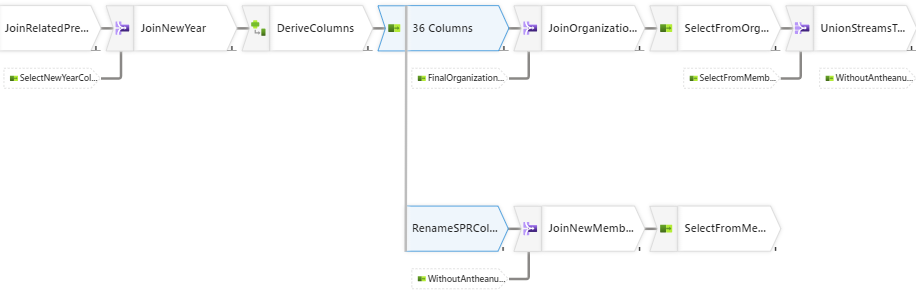
\includegraphics[width=1\textwidth]{./graphics/adf/bepalen_groep_3.png}
    \caption{Hernoemen van kolommen op ``new\_syndicalpremiumrequest'' en splitsing in twee apparte branches}
\end{figure}

Vervolgens worden bepaalde kolommen van naam hernoemt. Welke kolommen dit zijn is onbelangrijk voor deze transformatie. Wat wel belangrijk is dat de pipeline zich nu opsplitst in twee apparte branches. Dit doordat er 2 inner joins zullen gebeuren.

\begin{figure}[H]
    \centering
    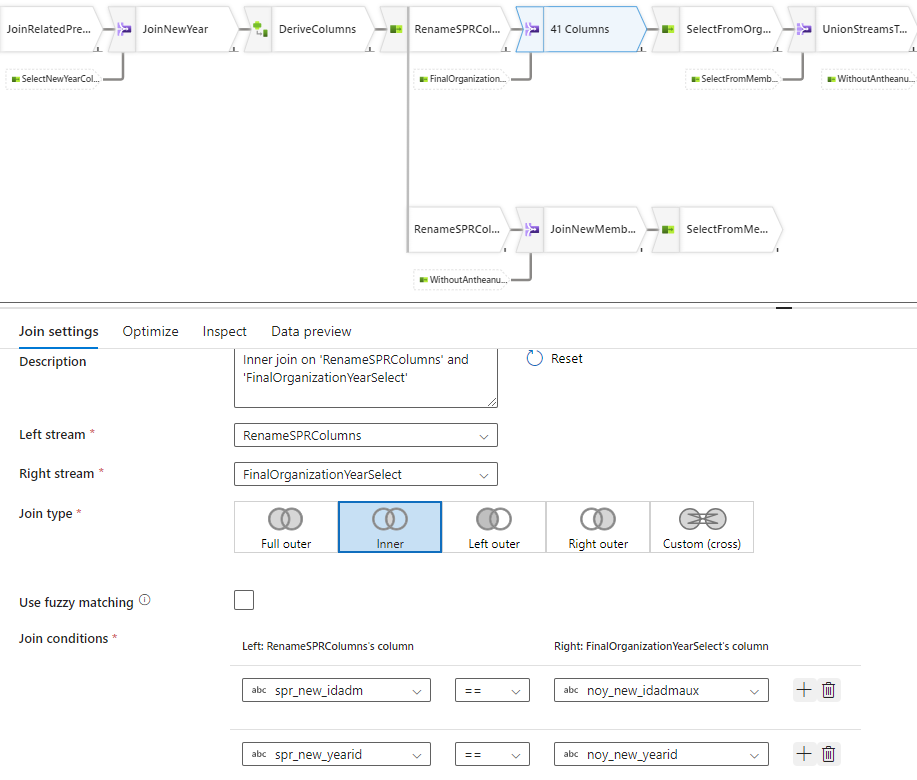
\includegraphics[width=0.9\textwidth]{./graphics/adf/bepalen_groep_4.png}
    \caption{Inner join van ``new\_organizationyear'' op de tabel ``new\_syndicalpremiumrequest''}
\end{figure}

Er gebeurt nu een inner join van de tabel ``new\_organizationyear'' op de tabel ``new\_syndicalpremiumrequest''. Hierbij wordt er aan de hand van IDADM en het id van het referentiejaar gejoind.

\begin{figure}[H]
    \centering
    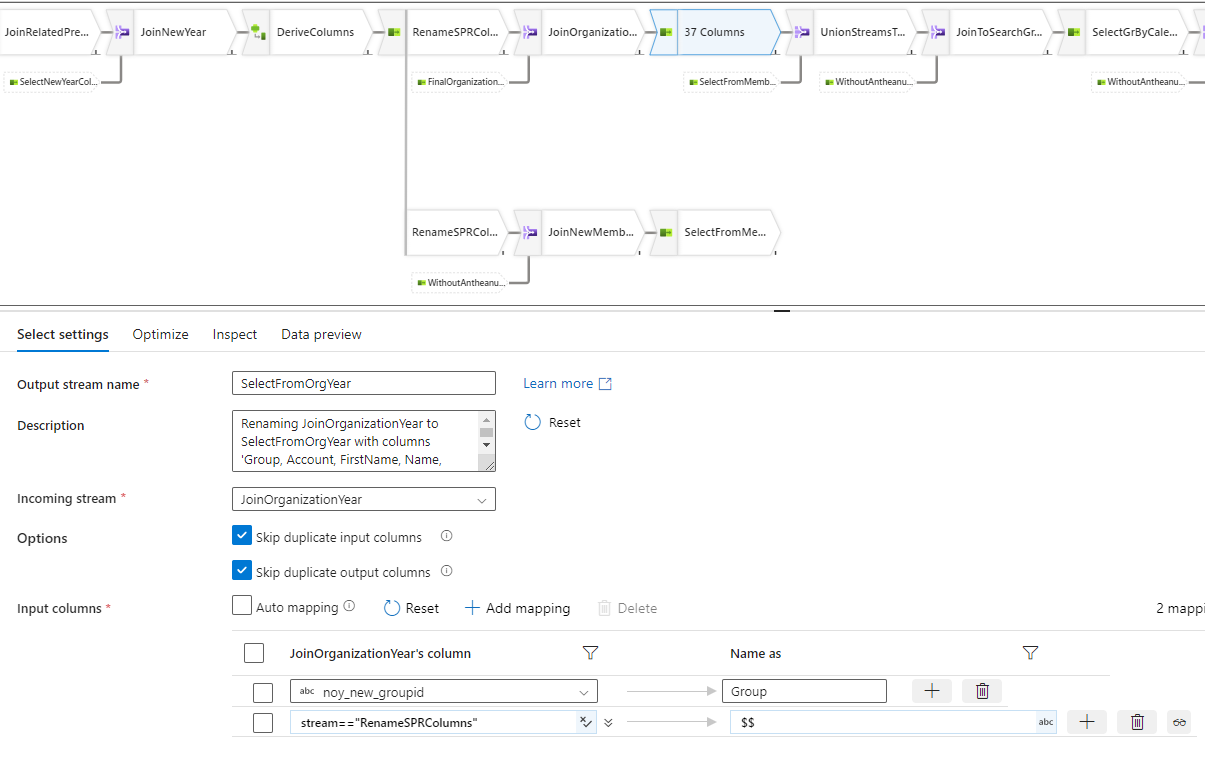
\includegraphics[width=1\textwidth]{./graphics/adf/bepalen_groep_5.png}
    \caption{Selecteren en hernoemen van kolommen op de tabel ``new\_syndicalpremiumrequest''}
\end{figure}

Vervolgens worden alle kolommen, die er voor de join waren, geselecteerd. Daarnaast wordt er één kolom ``noy\_new\_groupid'' geselecteerd en hernoemd naar ``Group''.

\begin{figure}[H]
    \centering
    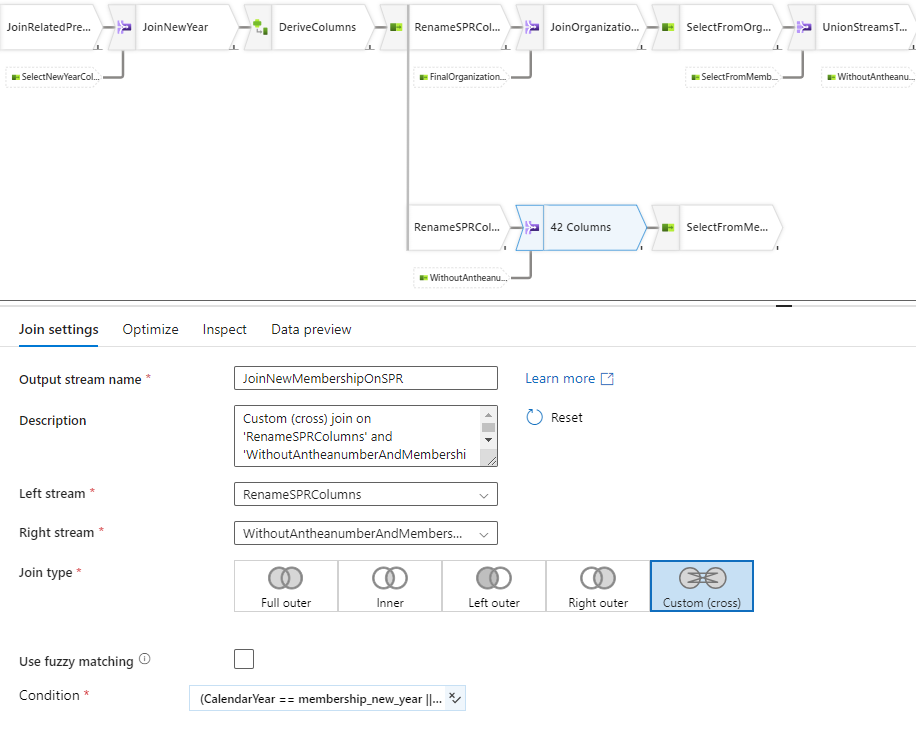
\includegraphics[width=0.8\textwidth]{./graphics/adf/bepalen_groep_6.png}
    \caption{Custom (cross) join van ``new\_membership'' op de tabel ``new\_syndicalpremiumrequest''}
\end{figure}

Bij de tweede branch wordt de tabel ``new\_membership'' gejoind op de tabel ``new\_syndicalpremiumrequest''. Er wordt gebruik gemaakt van een custom (cross) join doordat er OR condities gebruikt worden. De custom (cross) join is de enigste join die gebruik kan maken van OR condities binnen Azure Data Factory. Door deze condities, zal deze join werken net zoals een inner join. 

\begin{minted}{text}
    (CalendarYear == membership_new_year || EntryYear == membership_new_year || RefYear == membership_new_year) 
    && spr_new_personid == membership_new_personid
\end{minted}

In de conditie van de custom (cross) join wordt er vergeleken of CalendarYear, EntryYear of RefYear overeenkomt met het jaartal van de membership. Daarnaast wordt er ook gekeken of personid overeen komt. Het is belangrijk dat deze vergelijking op personid niet wordt vergeten aangezien de pipeline dan anders oneindig zal blijven runnen. 

\begin{figure}[H]
    \centering
    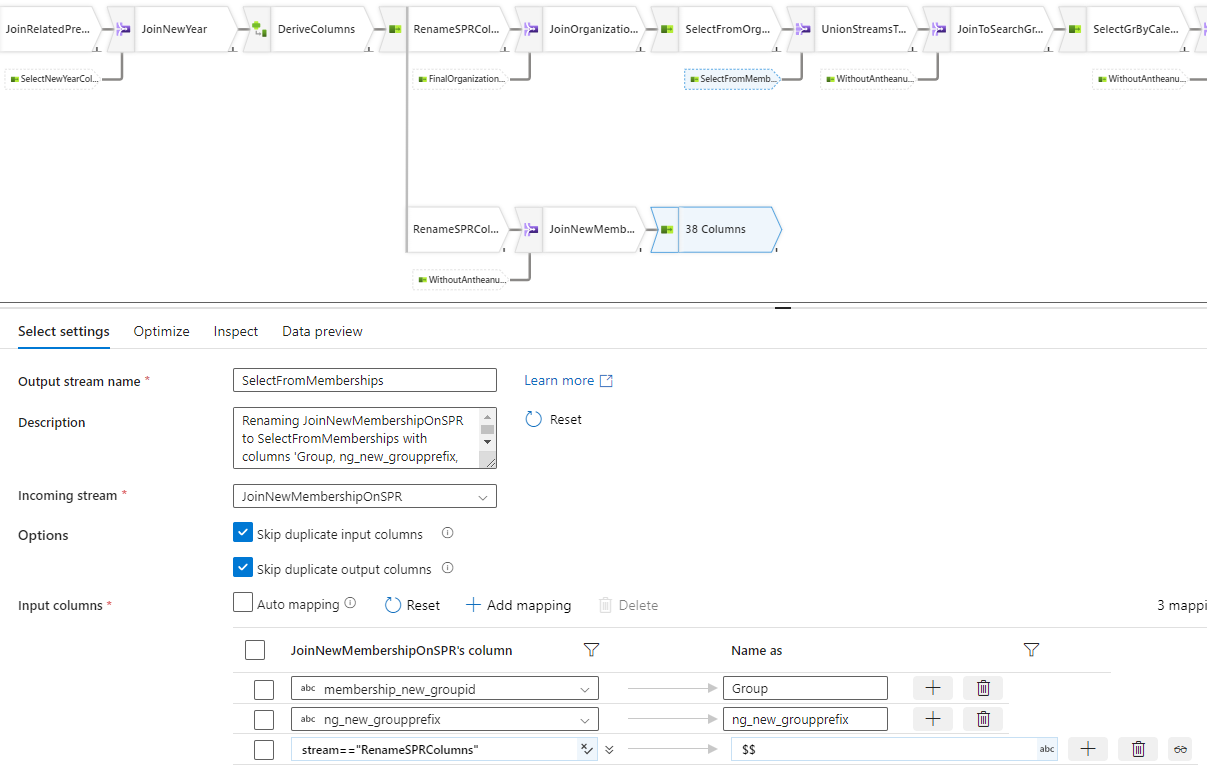
\includegraphics[width=1\textwidth]{./graphics/adf/bepalen_groep_8.png}
    \caption{Selecteren en hernoemen van kolommen op de tabel ``new\_syndicalpremiumrequest''}
    \label{fig:bepalengroep}
\end{figure}

Ook na deze join worden alle kolommen die er voor de join waren geselecteerd. Daarnaast wordt er één kolom ``membership\_new\_groupid'' geselecteerd en hernoemd naar ``Group''. Ten slotte wordt de kolom ``ng\_new\_groupprefix'' geselecteerd maar dit heeft te maken met een andere transformatie.

\begin{figure}[H]
    \centering
    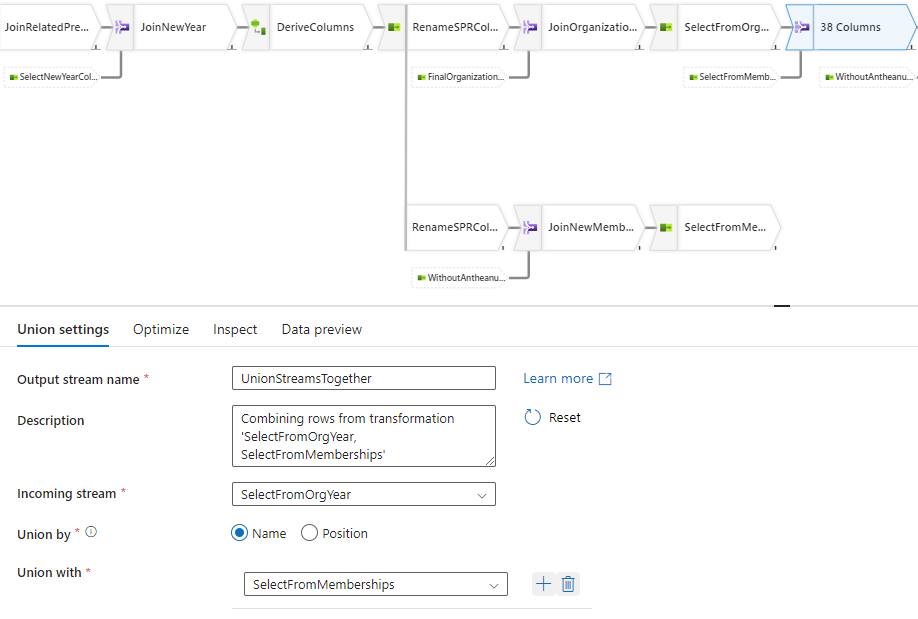
\includegraphics[width=1\textwidth]{./graphics/adf/bepalen_groep_9.png}
    \caption{Union van twee branches}
\end{figure}

Beide branches hebben nu dezelfde kolommen met een extra kolom ``Group''. Daarnaast heeft de onderste branch nog één extra kolom ``ng\_new\_groupprefix''. De beide branches worden samen gevoegd met behulp van een union. De bovenste branch die de kolom ``ng\_new\_groupprefix'' niet heeft zal voor deze kolom de waarde ``NULL'' krijgen in de records komende van deze branch. 

\begin{figure}[H]
    \centering
    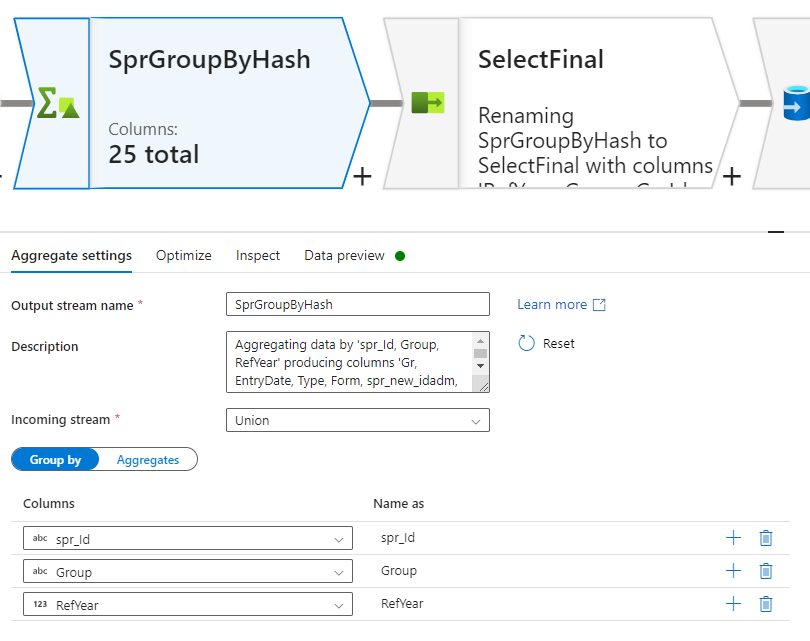
\includegraphics[width=0.8\textwidth]{./graphics/adf/group_by_1.png}
    \caption{Group by ``spr\_Id'', ``Group'' en ``RefYear'' in ``new\_syndicalpremiumrequest''}
    \label{fig:groupby}
\end{figure}

Om te voorkomen dat een premie twee keer in het zelfde bestand terecht komt voor een bepaalde groep en referentiejaar zal er op het einde van de pipeline gegroepeerd worden op basis van id van de premie, groep en referentiejaar.

\begin{figure}[H]
    \centering
    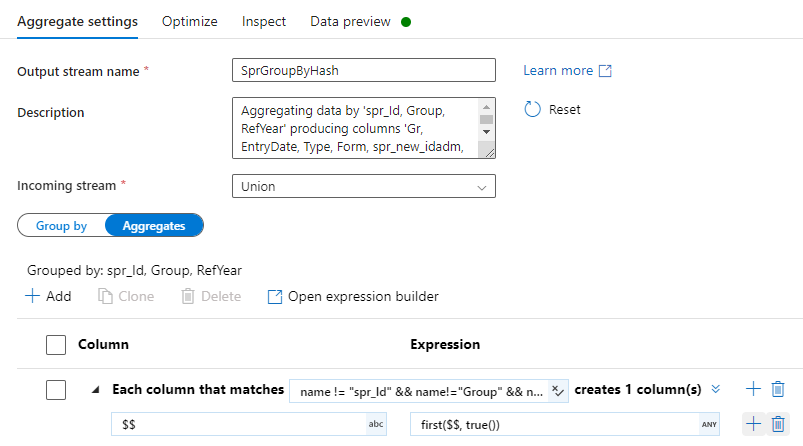
\includegraphics[width=0.8\textwidth]{./graphics/adf/group_by_2.png}
    \caption{Group by ``spr\_Id'', ``Group'' en ``RefYear'' in ``new\_syndicalpremiumrequest''}
\end{figure}

\begin{minted}{text}
    name != "spr_Id" && name != "Group" && name != "RefYear"
\end{minted}

Voor alle kolommen behalve de kolommen die in de ``Group by'' gebruikt worden zal de aggregatiefunctie ``first'' gebruikt worden. De tweede parameter ``true()'' wordt gebruikt om aan te geven dat ``NULL'' waardes genegeerd moeten worden. Dit zal dus resulteren in de eerste waarde die niet ``NULL'' is van de kolom groep. Indien alle waardes ``NULL'' zijn zal dit wel in ``NULL'' resulteren. \\

De premie heeft nu een id, een groep en een referentiejaar. Op basis hier van kan bepaald worden welke premie naar naar welk exportbestand voor een bepaalde groep en referentiejaar moet geëxporteerd worden.


% TODO group by uitleggen

\subsubsection{Bepalen van de kolom ``Gr'' voor een premie}

\begin{figure}[H]
    \centering
    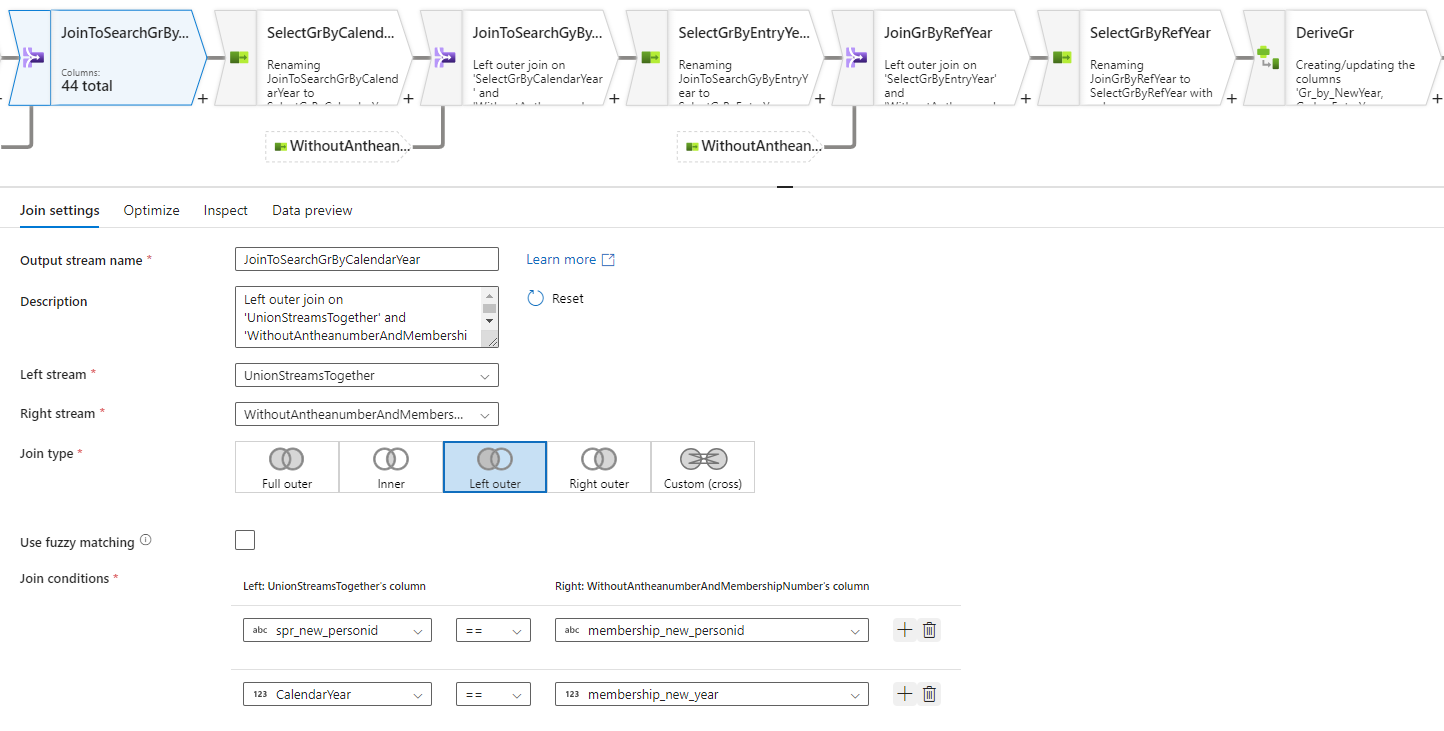
\includegraphics[width=1\textwidth]{./graphics/adf/gr_1.png}
    \caption{Joinen van de tabel ``new\_membership'' op de tabel ``new\_syndicalpremiumrequest''}
\end{figure}

De tabel ``new\_membership'' wordt gejoind op de tabel ``new\_syndicalpremiumrequest''. Dit gebeurd aan de hand van ``new\_personid'' en het kalenderjaar van de premie.

\begin{figure}[H]
    \centering
    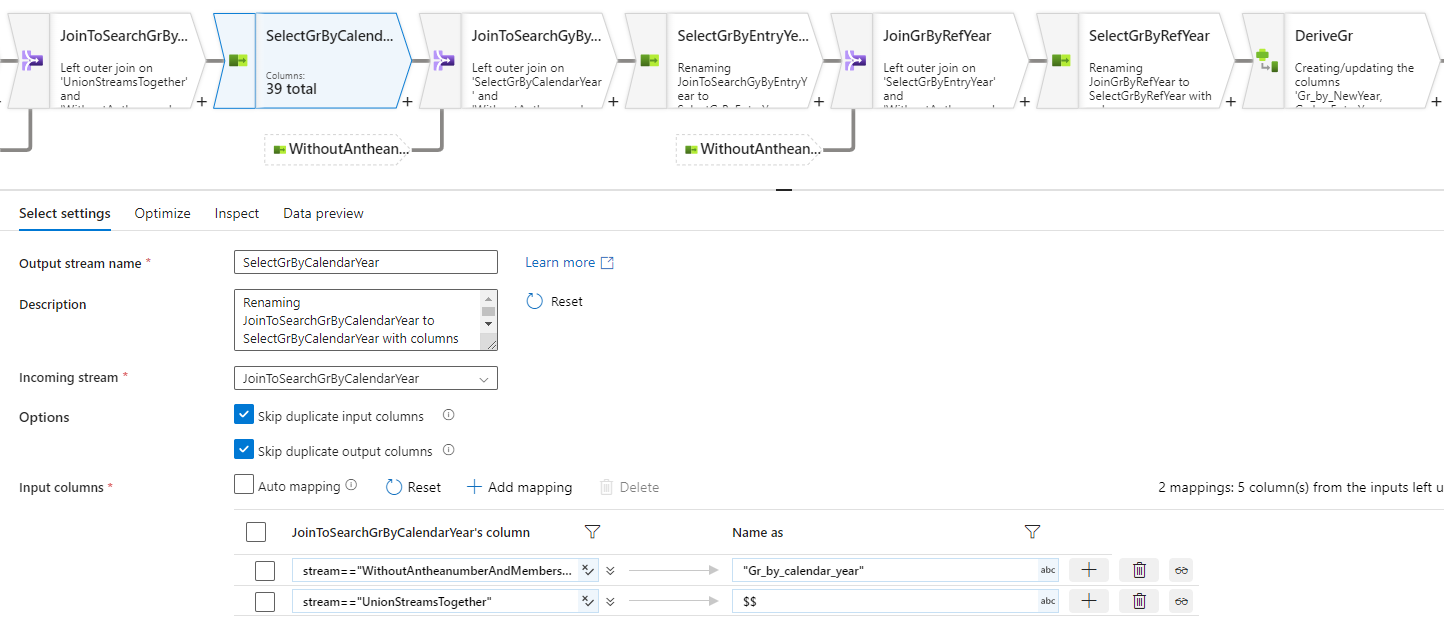
\includegraphics[width=1\textwidth]{./graphics/adf/gr_2.png}
    \caption{Selecteren van de juiste kolommen in ``new\_syndicalpremiumrequest''}
\end{figure}

De kolommen die reeds bestonden voor de join worden geselecteerd. Daarnaast wordt de kolom ``ng\_new\_groupprefix'' geselecteerd en hernoemd naar ``Gr\_by\_calendar\_year''.

\begin{figure}[H]
    \centering
    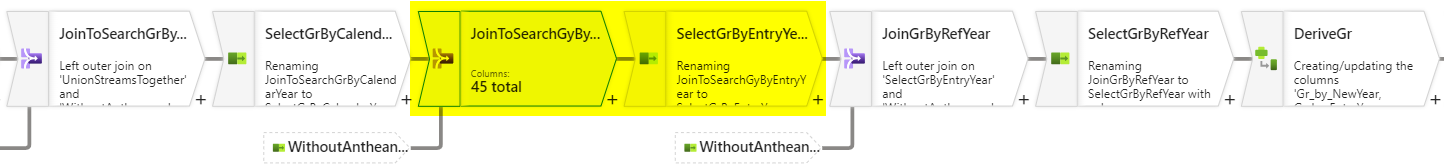
\includegraphics[width=1\textwidth]{./graphics/adf/gr_3.png}
    \caption{Herhalen van transformaties}
\end{figure}

Dezelfde transformaties gebeuren opnieuw maar deze keer aan de hand van ``EntryYear''. Ook hier worden de reeds bestaande kolommen geselecteerd en wordt de nieuwe kolom ``ng\_new\_groupprefix'' hernoemd naar ``Gr\_by\_EntryYear''.

\begin{figure}[H]
    \centering
    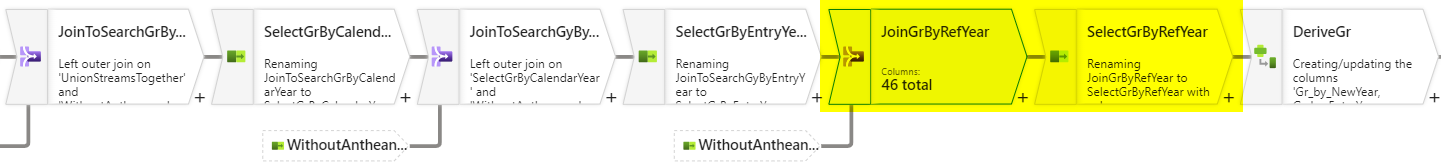
\includegraphics[width=1\textwidth]{./graphics/adf/gr_4.png}
    \caption{Herhalen van transformaties}
\end{figure}

Ook voor ``RefYear'' zullen deze transformaties gebeuren, resulterend in een nieuwe kolom ``Gr\_by\_RefYear''.

\begin{figure}[H]
    \centering
    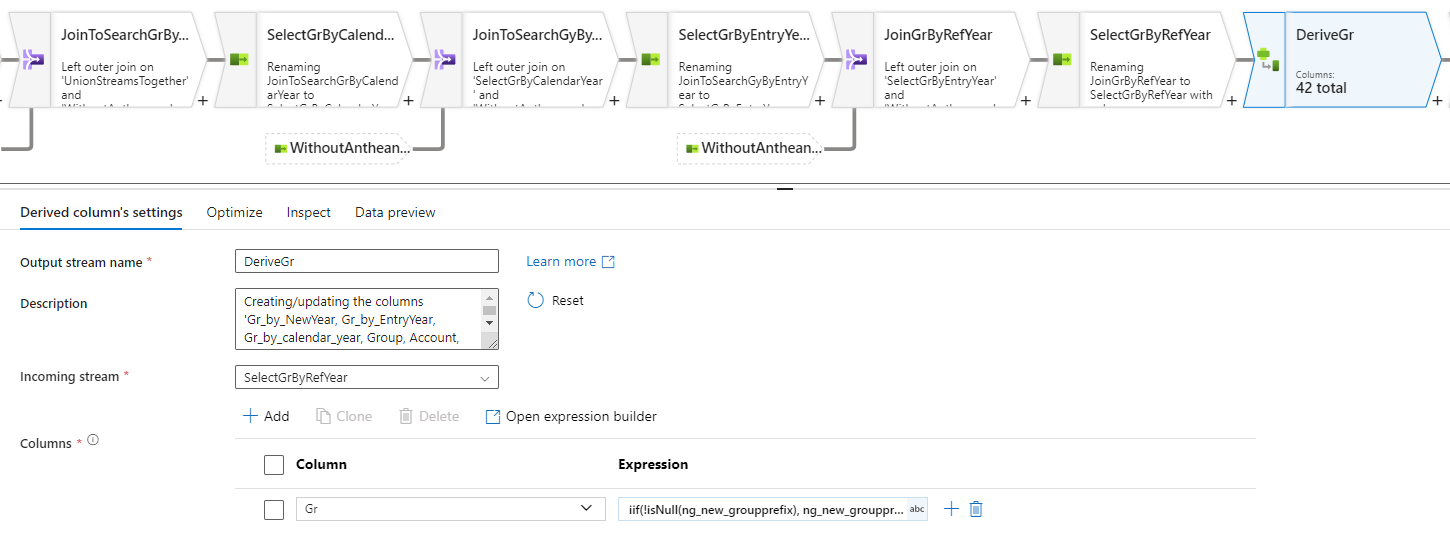
\includegraphics[width=1\textwidth]{./graphics/adf/gr_5.png}
    \caption{Bepalen van ``Gr'' in ``new\_syndicalpremiumrequest''}
\end{figure}

We hebben nu een group prefix reeds komende uit een andere transformatie \ref{fig:bepalengroep} en group prefixes komende uit de joins die we hebben uitgevoerd.

\begin{minted}{text}
iif(!isNull(ng_new_groupprefix), ng_new_groupprefix, 
    iif(!isNull(Gr_by_calendar_year), Gr_by_calendar_year,
        iif(!isNull(Gr_by_EntryYear), Gr_by_EntryYear,
            iif(!isNull(Gr_by_NewYear), Gr_by_RefYear, toString(null())))))
\end{minted}

Om de kolom ``Gr'' te bepalen zal er gezocht worden naar de eerste kolom die niet ``NULL'' is startende van uit ``ng\_new\_groupprefix'' waarbij er vervolgens gekeken wordt naar ``Gr\_by\_calendar\_year'', `Gr\_by\_EntryYear` en `Gr\_by\_NewYear`.

Ook voor deze transformatie is het belangrijk dat er gegroepeerd wordt zoals bij Figuur \ref{fig:groupby} om te voorkomen dat dezelfde premie twee keer in een groep voor een bepaald referentiejaar terecht komt.

\subsubsection{Bepalen van de kolommen ``AntheaNumber'' en ``MembershipNumber'' voor een premie}

\begin{figure}[H]
    \centering
    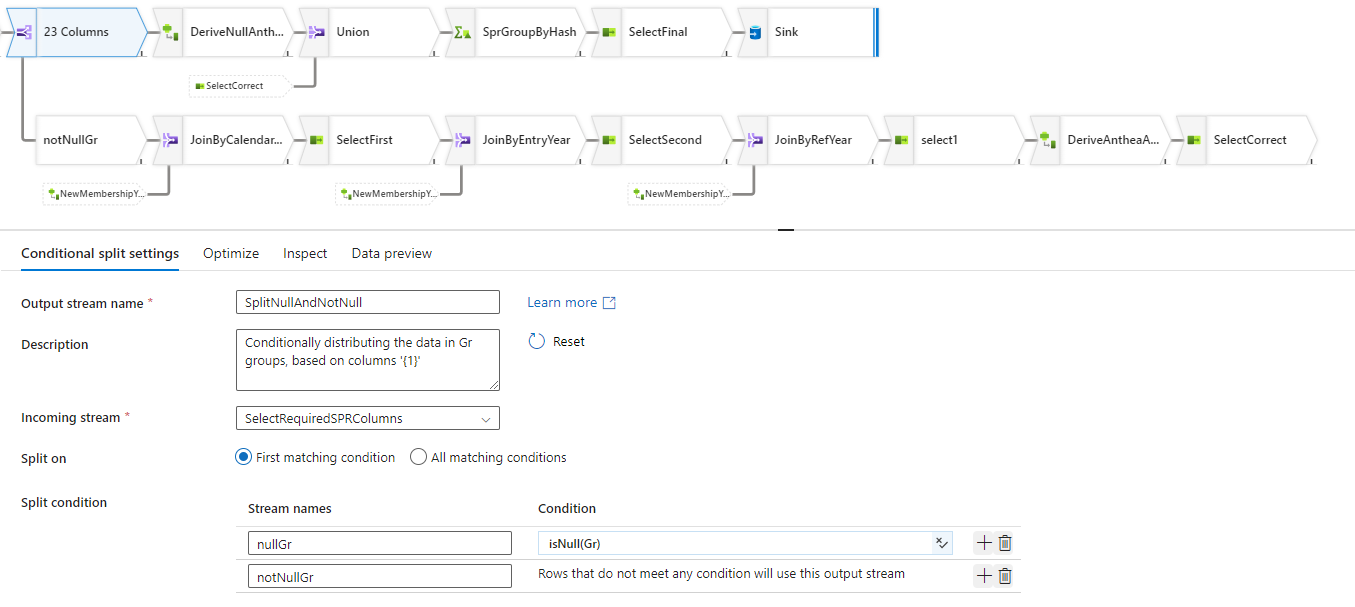
\includegraphics[width=1\textwidth]{./graphics/adf/member_1.png}
    \caption{Conditional split op de tabel ``new\_syndicalpremiumrequest''}
\end{figure}

De pipeline zal splitten in twee branches met behulp van een conditional split. Alle rijen waarbij de kolom ``Gr'' ``NULL'' is, zullen boven verder gaan. Alle rijen waarbij de kolom ``Gr'' niet ``NULL'' zijn, zullen onderaan verder gaan.

\begin{figure}[H]
    \centering
    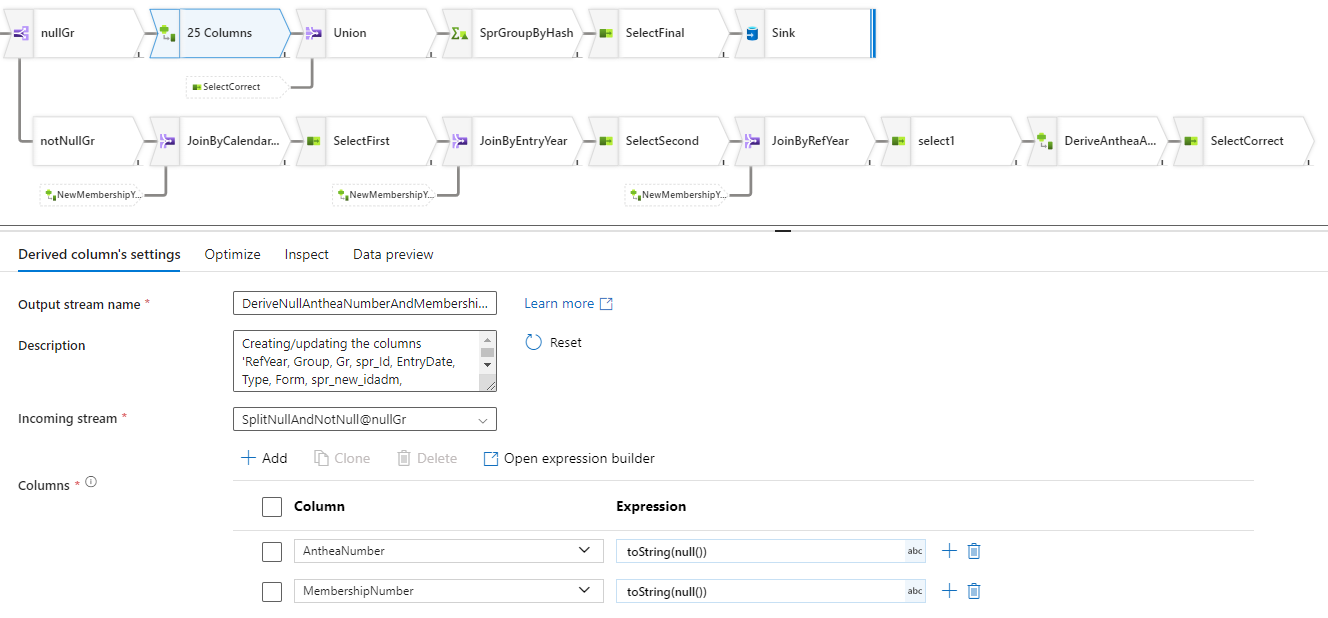
\includegraphics[width=1\textwidth]{./graphics/adf/member_2.png}
    \caption{Derive ``AntheaNumber'' en ``MembershipNumber'' op de tabel ``new\_syndicalpremiumrequest''}
\end{figure}

Voor de rijen waarbij de kolom ``Gr'' ``NULL'' was, zullen de kolommen ``AntheaNumber'' en ``MembershipNumber'' ook ``NULL'' zijn.

\begin{figure}[H]
    \centering
    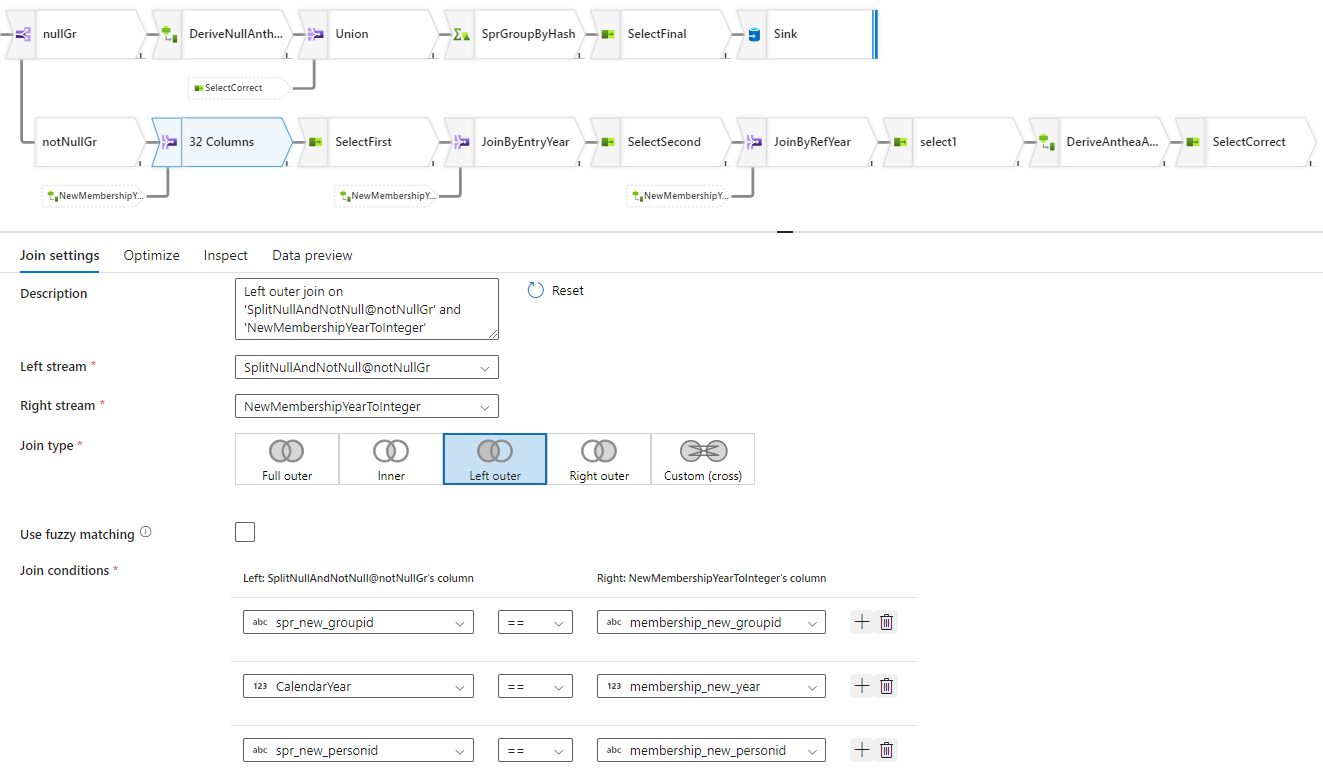
\includegraphics[width=1\textwidth]{./graphics/adf/member_3.png}
    \caption{Join van de tabel ``new\_membership'' op de tabel ``new\_syndicalpremiumrequest'' aan de hand van ``new\_groupid'', ``new\_personid'' en ``CalendarYear''}
\end{figure}

Voor de rijen waarbij de kolom ``Gr'' niet ``NULL'' was, zal de tabel ``new\_membership'' hier op gejoind worden. Hierbij wordt er gebruik gemaakt van ``group\_id'', ``new\_personid'' en ``CalendarYear''.

\begin{figure}[H]
    \centering
    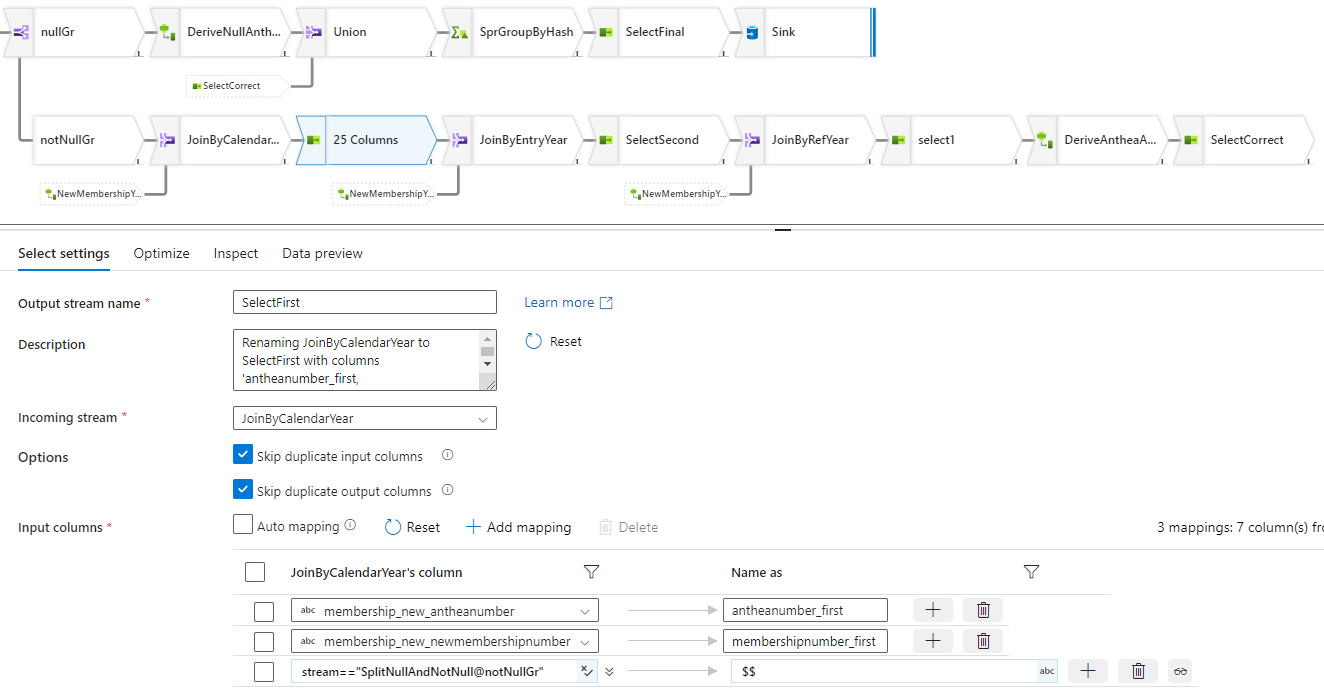
\includegraphics[width=1\textwidth]{./graphics/adf/member_4.png}
    \caption{Select op de tabel ``new\_syndicalpremiumrequest''}
\end{figure}

Alle kolommen die er voor de join waren zullen opnieuw geselecteerd worden. Daarnaast worden ``membership\_new\_antheanumber'' en ``membership\_new\_newmembershipnumber'' geselecteerd en hernoemd naar ``antheanumber\_first'' en ``membershipnumber\_first''.

\begin{figure}[H]
    \centering
    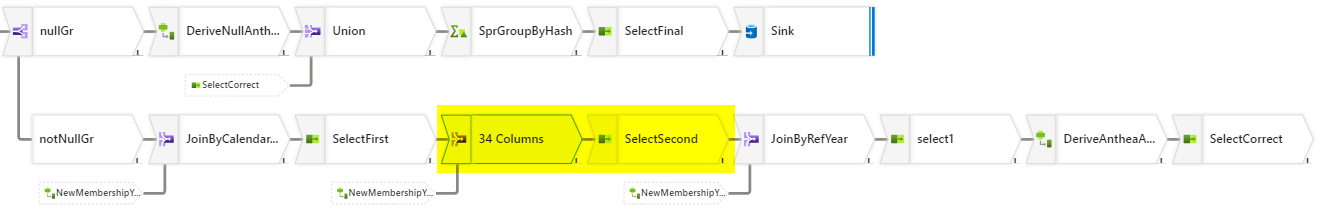
\includegraphics[width=1\textwidth]{./graphics/adf/member_5.png}
    \caption{Join van de tabel ``new\_membership'' op de tabel ``new\_syndicalpremiumrequest'' aan de hand van ``new\_groupid'', ``new\_personid'' en ``EntryYear''}
\end{figure}

De vorige twee transformatie gebeuren opnieuw maar deze keer wordt er gebruik gemaakt van ``EntryYear'' in plaats van ``CalendarYear''. Daarnaast worden de kolommen ``membership\_new\_antheanumber'' en ``membership\_new\_newmembershipnumber'' deze keer hernoemd naar ``antheanumber\_second'' en ``membershipnumber\_second''.

\begin{figure}[H]
    \centering
    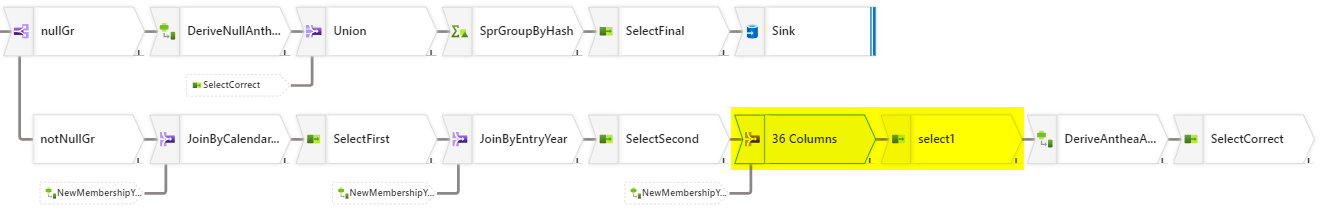
\includegraphics[width=1\textwidth]{./graphics/adf/member_6.png}
    \caption{Join van de tabel ``new\_membership'' op de tabel ``new\_syndicalpremiumrequest'' aan de hand van ``new\_groupid'', ``new\_personid'' en ``RefYear''}
\end{figure}

Ook zal voor ``RefYear'' in plaats van ``CalendarYear'' deze transformaties opnieuw gebeuren. Deze keer met de kolommen ``antheanumber\_third'' en ``membershipnumber\_third'' als resultaat.

\begin{figure}[H]
    \centering
    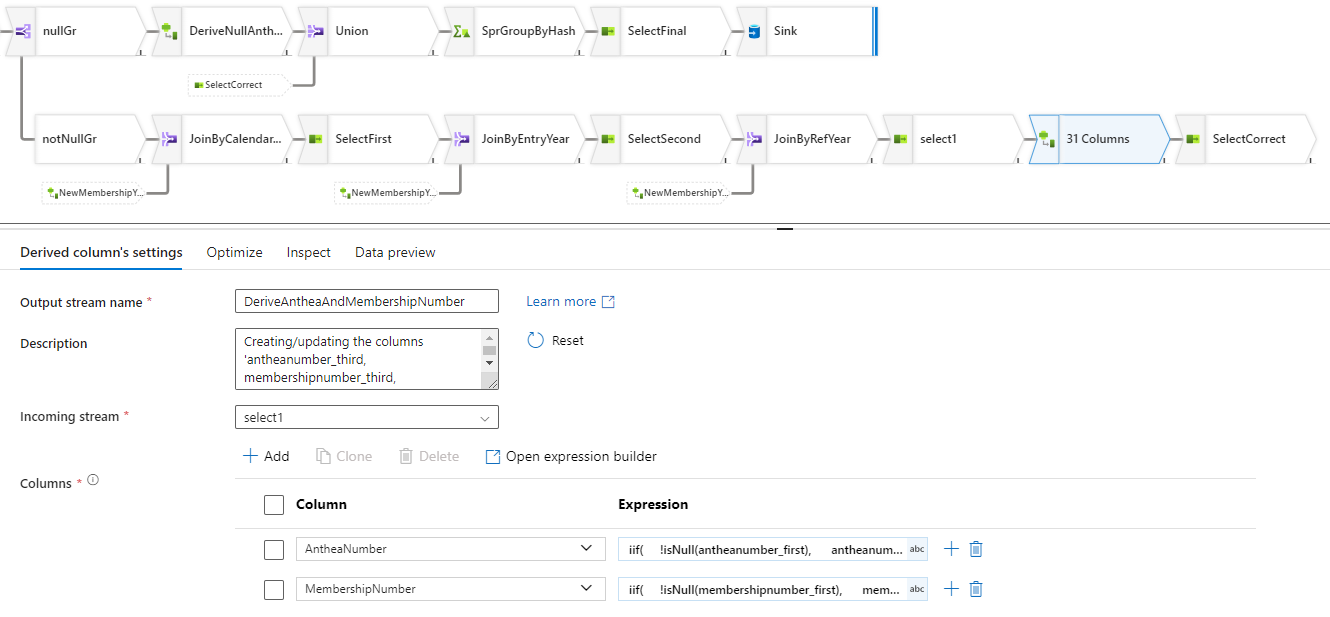
\includegraphics[width=1\textwidth]{./graphics/adf/member_7.png}
    \caption{Derive van kolommen ``AntheaNumber'' en ``MembershipNumber'' op de tabel ``new\_syndicalpremiumrequest''}
\end{figure}

De kolommen ``AntheaNumber'' en ``MembershipNumber'' worden nu berekent.

\begin{minted}{text}
iif(!isNull(antheanumber_first), antheanumber_first,      
    iif(!isNull(antheanumber_second), antheanumber_second,
        iif(!isNull(antheanumber_third), antheanumber_third, toString(null()))))
\end{minted}

Wanneer het antheanummer van de eerste join niet ``NULL'' is zal deze gebruikt worden, anders zal er gekeken worden of de tweede niet ``NULL'' is. Als de tweede ``NULL'' is zal de derde gebruikt worden. Indien de derde ook ``NULL'' is zal dit resulteren in ``NULL'' als waarde voor de kolom ``AntheaNumber''.

\begin{minted}{text}
iif(!isNull(membershipnumber_first), membershipnumber_first, 
    iif(!isNull(membershipnumber_second), membershipnumber_second,         
        iif(!isNull(membershipnumber_third), membershipnumber_third, toString(null()))))
\end{minted}

Ook de kolom ``MembershipNumber'' wordt op dezelfde manier berekent.

\begin{figure}[H]
    \centering
    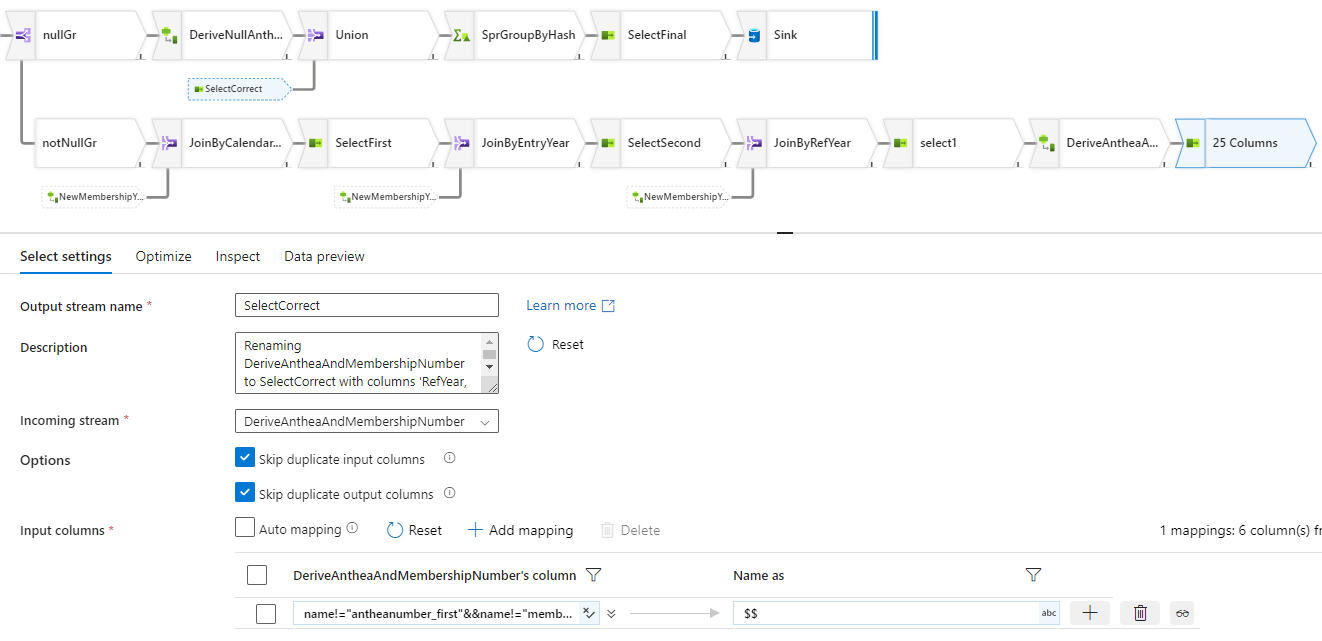
\includegraphics[width=1\textwidth]{./graphics/adf/member_8.png}
    \caption{Verwijderen van onnodige kolommen op de tabel ``new\_syndicalpremiumrequest''}
\end{figure}

De kolommen die niet nodig zijn worden verwijderd.

\begin{figure}[H]
    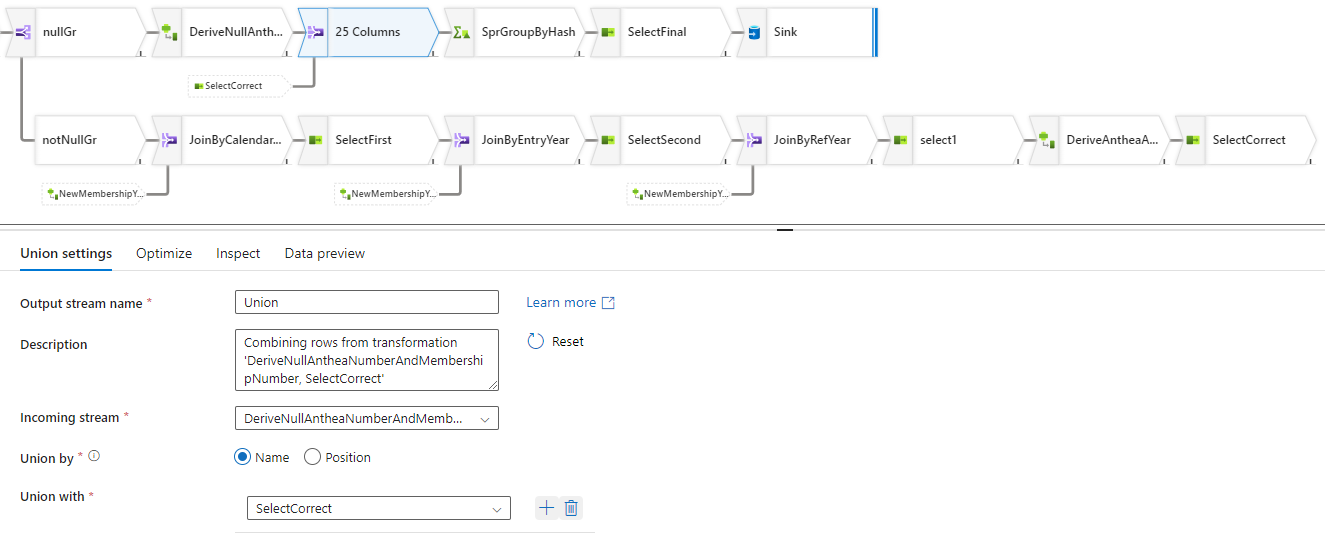
\includegraphics[width=1\textwidth]{./graphics/adf/member_9.png}
    \caption{Union van twee streams}
\end{figure}

Beide streams worden nu samen gevoegd met behulp van een union.

En ten slotte is het ook voor deze transformatie belangrijk dat er gegroepeerd wordt zoals bij Figuur \ref{fig:groupby} om te voorkomen dat dezelfde premie twee keer in een groep voor een bepaald jaartal terecht komt.

\subsection{Schrijven van data naar Azure Data Lake}

\begin{figure}[H]
    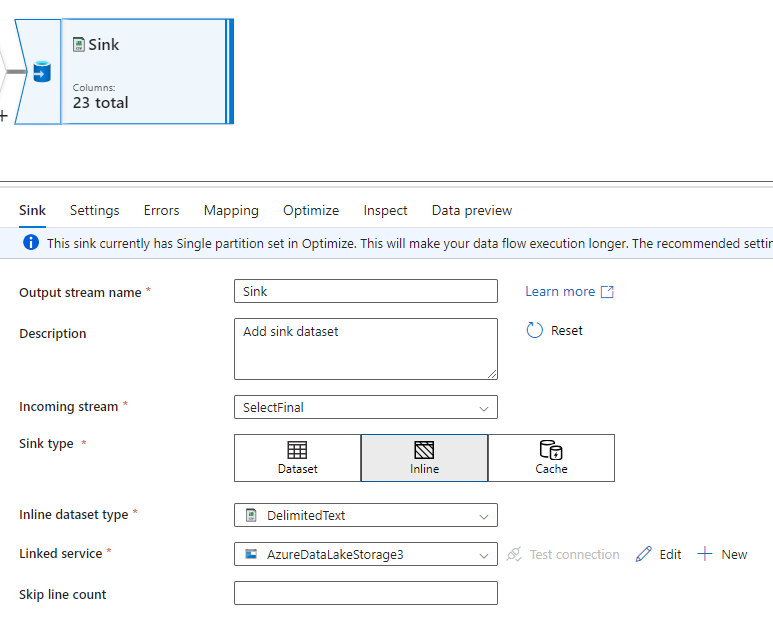
\includegraphics[width=1\textwidth]{./graphics/adf/sink.png}
    \caption{Sink in Azure Data Factory}
\end{figure}

Voor het schrijven van data naar Azure Data Lake wordt er gebruik gemaakt van een sink. Deze maakt ook gebruik van de Linked Service aangemaakt in Figuur~\ref{fig:linked-service}. Als ``Inline dataset type'' is hierbij gekozen voor ``DelimitedText'' zodat de resulterende output een CSV bestand is. Belangrijk is dat voor de proof-of-concepts één enkel CSV bestand geschreven wordt, hierdoor staat ``Partition option'' op ``Single partition''. 

\section{Azure Databricks}

\subsection{Opzet van resources}

Door in Microsoft Azure naar Databricks te navigeren kan er een nieuwe Azure Databricks workspace aangemaakt worden.

\begin{figure}[H]
    \centering
    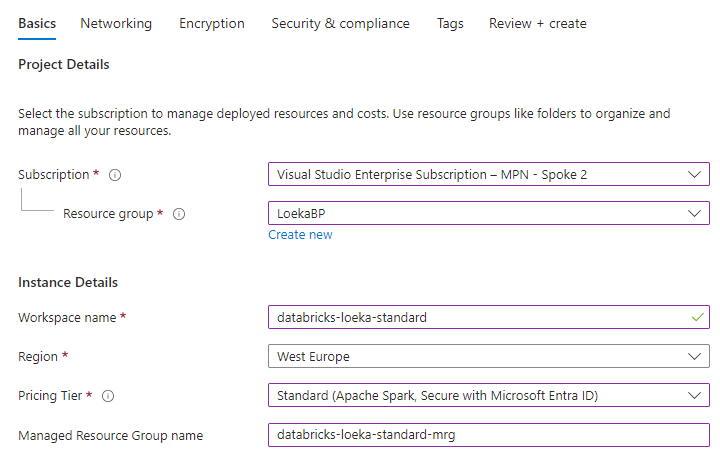
\includegraphics[width=1\textwidth]{./graphics/databricks/initial_2.png}
    \caption{Configuratie van Azure Databricks}
    \label{fig:conf-databricks}
\end{figure}

Bij het aanmaken van databricks moet er een subscription en resource group gekozen worden. Er kan een nieuwe resource group aangemaakt worden of een reeds bestaande gekozen worden. Daarnaast moet er een naam, gewenste regio en pricing tier gekozen worden. Als pricing tier kiezen we hier voor ``Standard'' doordat we geen gebruik gaan maken van Premium features. Ten slotte kan er ook een Managed Resource Group name gekozen worden. Deze resource group houdt alle resource bij die databricks nodig heeft, zoals bijvoorbeeld virtual machines, storage accounts en virtual networks.

\begin{figure}[H]
    \centering
    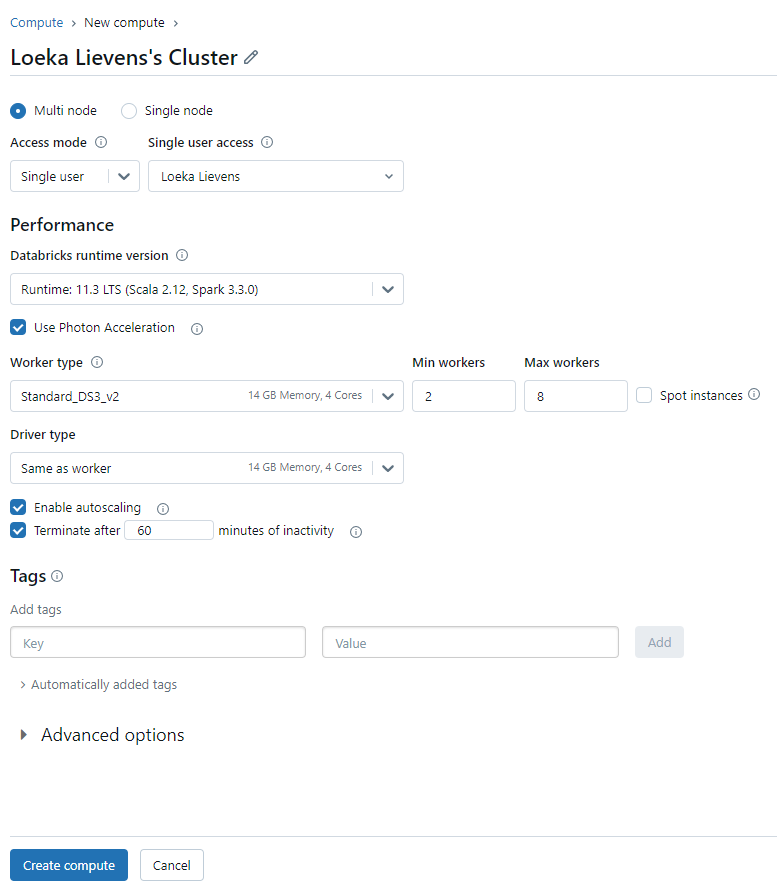
\includegraphics[width=0.9\textwidth]{./graphics/databricks/initial_5.png}
    \caption{Configuratie van compute resource}
\end{figure}

Voordat notebooks en jobs uitgevoerd kunnen worden zal er eerst een compute resource aangemaakt moeten worden. Hierbij zal de databricks runtime version op 11.3 LTS gezet moeten worden zodat we Apache Spark 3.3.0 kunnen gebruiken. Dit omdat we gebruik gaan maken van ``spark-cdm-connector''. Ook hebben we ingesteld dat de cluster zichzelf zal uitschakelen na 60 minuten om onnodige kosten te voorkomen.

\begin{figure}[H]
    \centering
    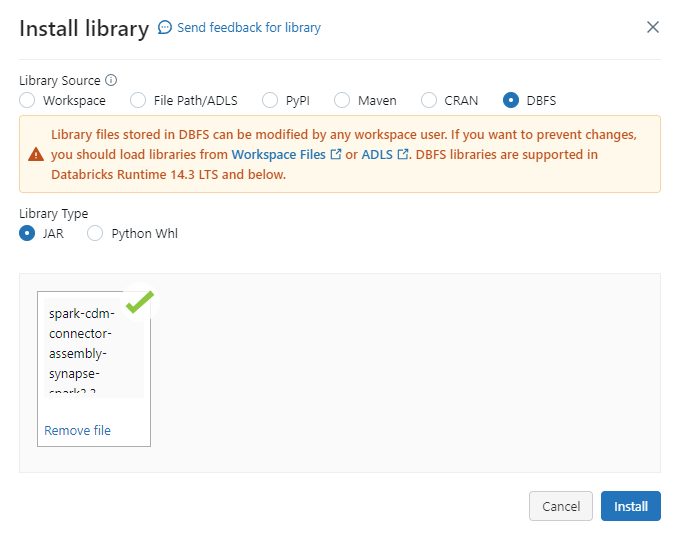
\includegraphics[width=1\textwidth]{./graphics/databricks/initial_6.png}
    \caption{Installatie van ``spark-cdm-connector''}
\end{figure}

Ten slotte moet de \href{https://github.com/Azure/spark-cdm-connector/releases/tag/spark3.3-1.19.5}{jar file} van ``spark-cdm-connector'' geïnstalleerd worden in het aangemaakte compute resource om gebruik te kunnen maken van het Common Data Model in onze pipeline.

\subsection{Collaboration en source control}

\subsubsection{Management en permissions}

\begin{figure}[H]
    \centering
    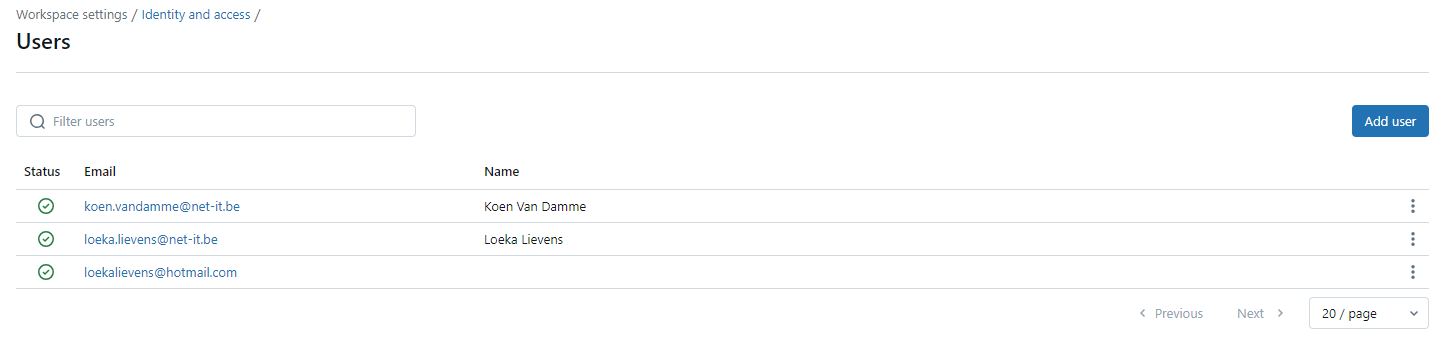
\includegraphics[width=1\textwidth]{./graphics/databricks/management_permissions_1.png}
    \caption{Gebruikers toevoegen/verwijderen in Azure Databricks}
\end{figure}

Gebruikers die behoren tot het AAD directory van de Azure Databricks environment kunnen makkelijk toegevoegd worden met behulp van het e-mailadres van de gebruiker.

\begin{figure}[H]
    \centering
    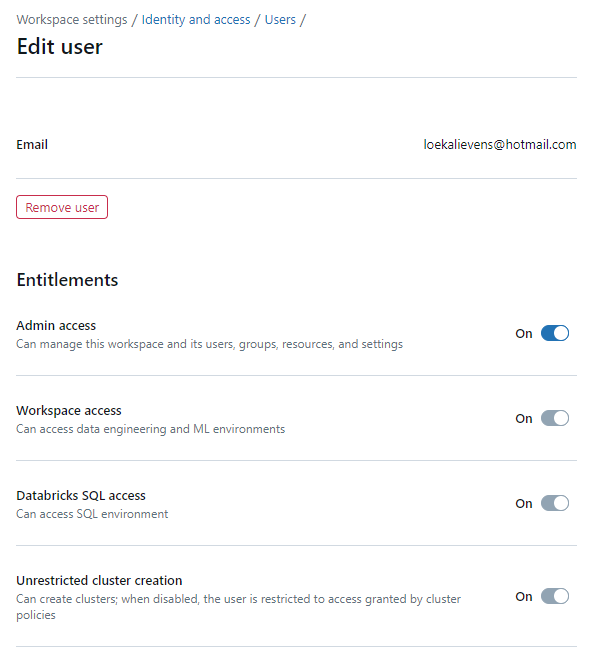
\includegraphics[width=0.6\textwidth]{./graphics/databricks/management_permissions_2.png}
    \caption{Rechten wijzigen van gebruikers in Azure Databricks}
\end{figure}

Rechten van gebruikers kunnen gewijzigd worden.

\begin{figure}[H]
    \centering
    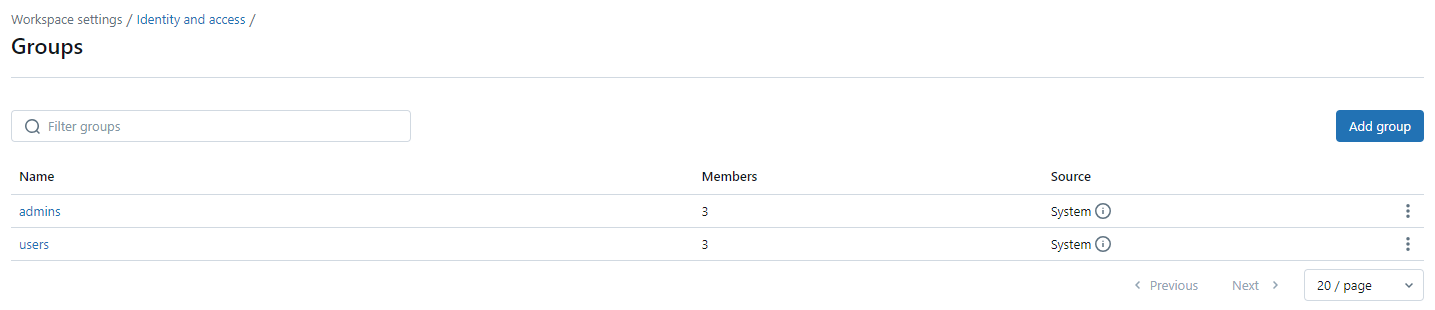
\includegraphics[width=0.9\textwidth]{./graphics/databricks/management_permissions_3.png}
    \caption{Groepen toevoegen of verwijderen in Azure Databricks}
\end{figure}

Er kunnen groepen toegevoegd of verwijderd worden aan Azure Databricks. Gebruikers kunnen dan aan deze groepen toegevoegd worden. Dit vereenvoudigt het om toegang toe te wijzen aan werkruimten, gegevens en andere objecten.

\subsubsection{Source control}

Databricks folders is een visuele Git client binnen Azure Databricks om gebruik te kunnen maken van source control.

\begin{figure}[H]
    \centering
    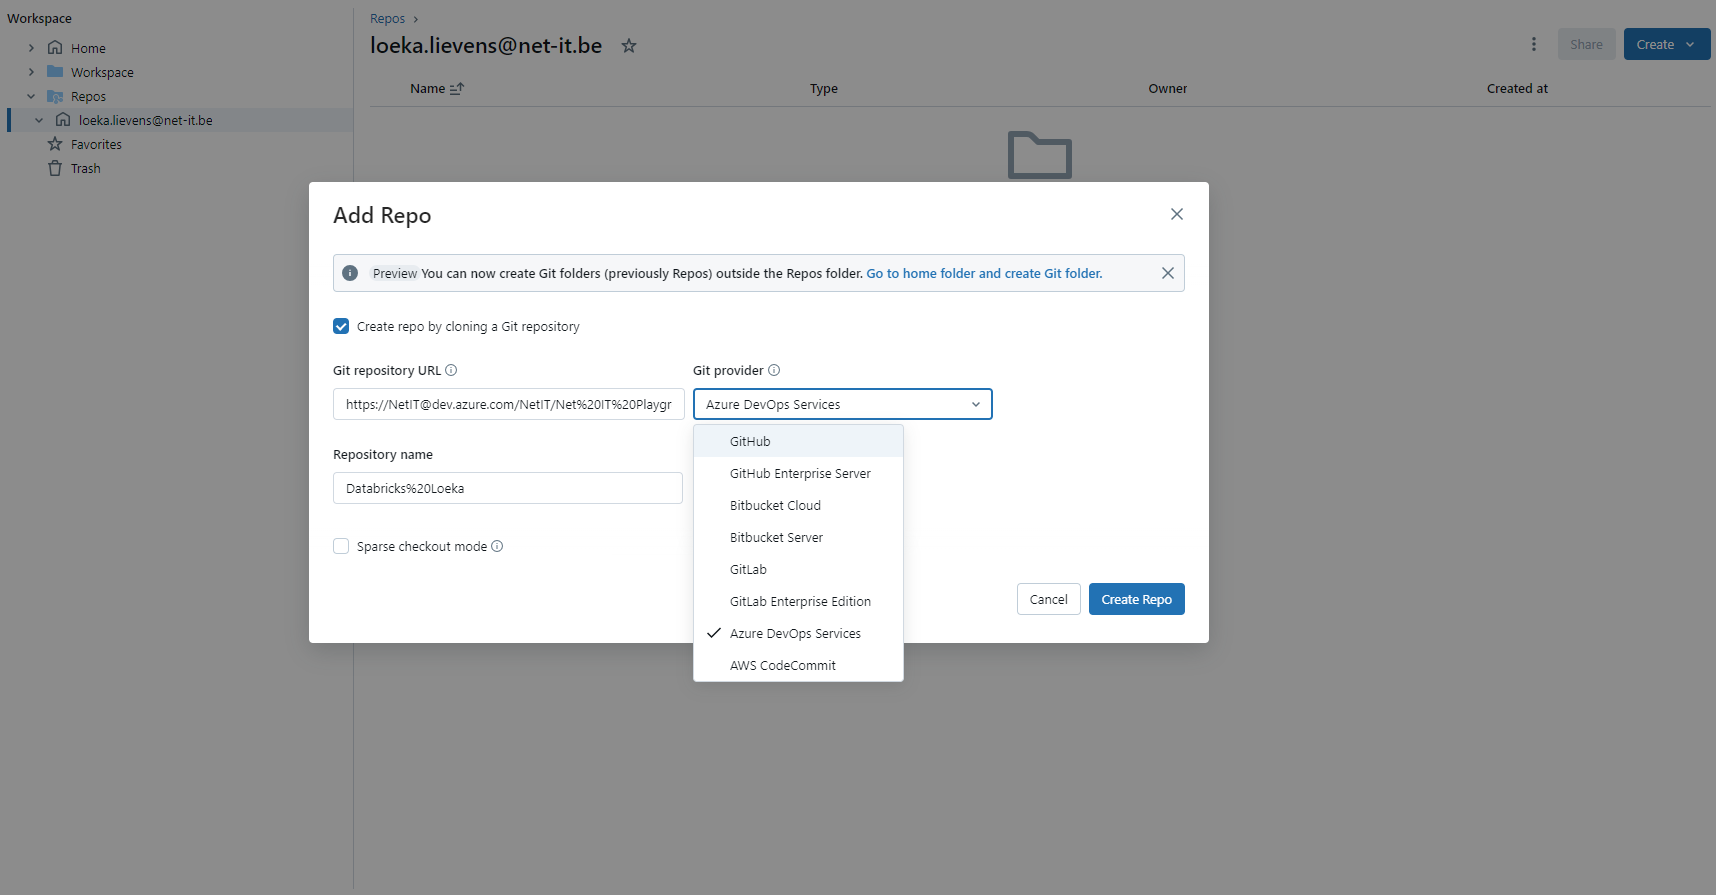
\includegraphics[width=1\textwidth]{./graphics/databricks/git_1.png}
    \caption{Clone Git repository in Databricks folders}
\end{figure}

Het geeft de optie om verschillende Git providers te gaan gebruiken. Doordat er binnen Net IT gewerkt wordt met Azure DevOps Services zal hier voor gekozen worden.

\begin{figure}[H]
    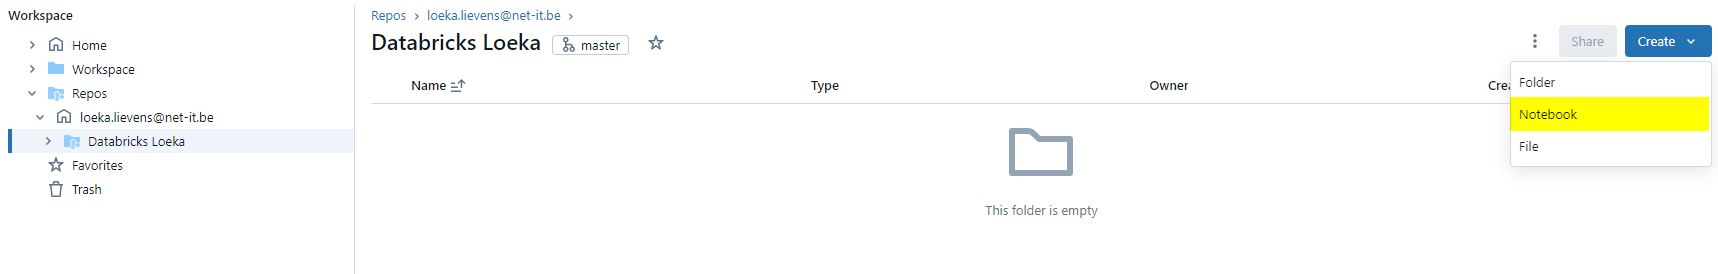
\includegraphics[width=1\textwidth]{./graphics/databricks/git_2.png}
    \caption{Aanmaken van een notebook in databricks}
\end{figure}

Ter illustratie zal er een voorbeeld notebook aangemaakt worden.

\begin{figure}[H]
    \centering
    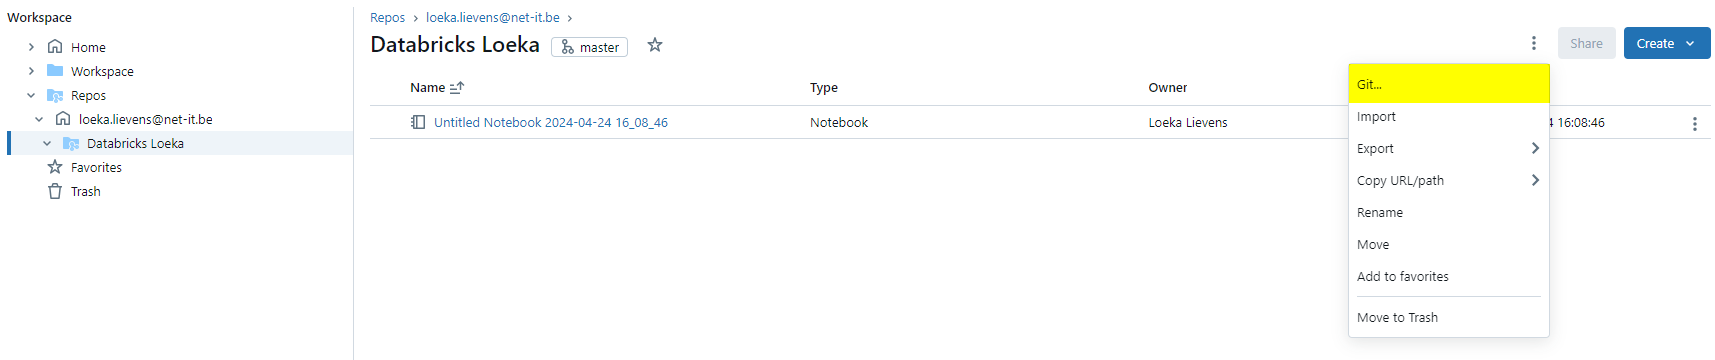
\includegraphics[width=1\textwidth]{./graphics/databricks/git_3.png}
    \caption{Commit en push in Databricks}
\end{figure}

\begin{figure}[H]
    \centering
    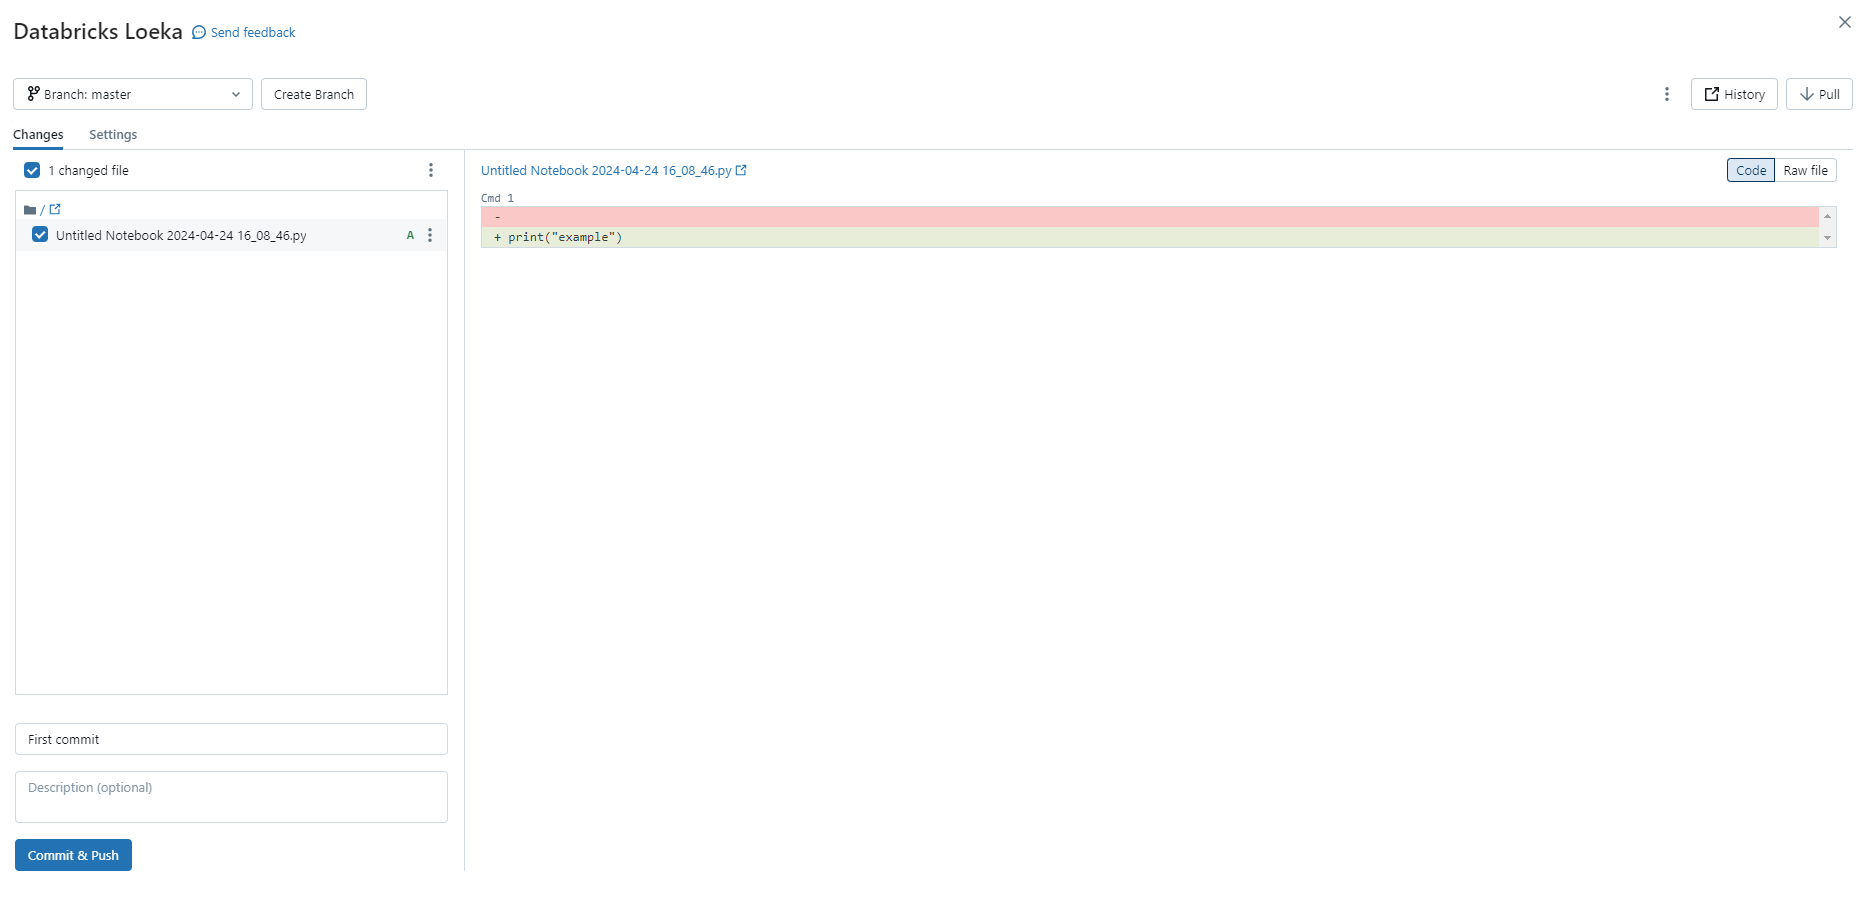
\includegraphics[width=1\textwidth]{./graphics/databricks/git_4.png}
    \caption{Commit en push in Databricks}
\end{figure}

Deze notebook kan dan gecommit worden naar Git.

\pagebreak

\subsection{IDE integratie}

Met behulp van Databricks Connect kan er vanuit Visual Studio Code, PyCharm, RStudio Desktop, IntelliJ IDEA, notebook servers en andere applicaties geconnecteerd worden met Databricks clusters. Hierdoor kan bijvoorbeeld Python-code zowel lokaal als op Databricks clusters uitgevoerd worden. Daarnaast kan code ook gesynchroniseerd worden met een Databricks workspace. Ook kan er makkelijk gedebugged worden met behulp van Databricks Connect.

\subsection{Infrastructure as code (IaC)}

Ook Azure Databricks kan met behulp van Azure Resource Manager (ARM) templates aangemaakt worden. Hierbij is het grote verschil wel dat bijvoorbeeld het aanmaken van clusters niet ondersteund worden. Er kan wel gebruik gemaakt worden van terraform om dit te implementeren. Daarnaast kan er ook gebruik gemaakt worden van Databricks Asset Bundles (DABs). Deze maakt het mogelijk om CI/CD te gaan implementeren met behulp van YAML syntax. Een bundle bevat dus de nodige cloud infrastructuur en workspace configurations, source files zoals bijvoorbeeld notebooks en Python files, definities voor Databricks resources en unit tests en integration tests. Met behulp van de Databricks CLI kunnen bundles gepubliceerd worden van uit de command line. 

\subsection{Ophalen van data uit Azure Data Lake}
\label{sec:ophalen}

\begin{figure}[H]
    \centering
    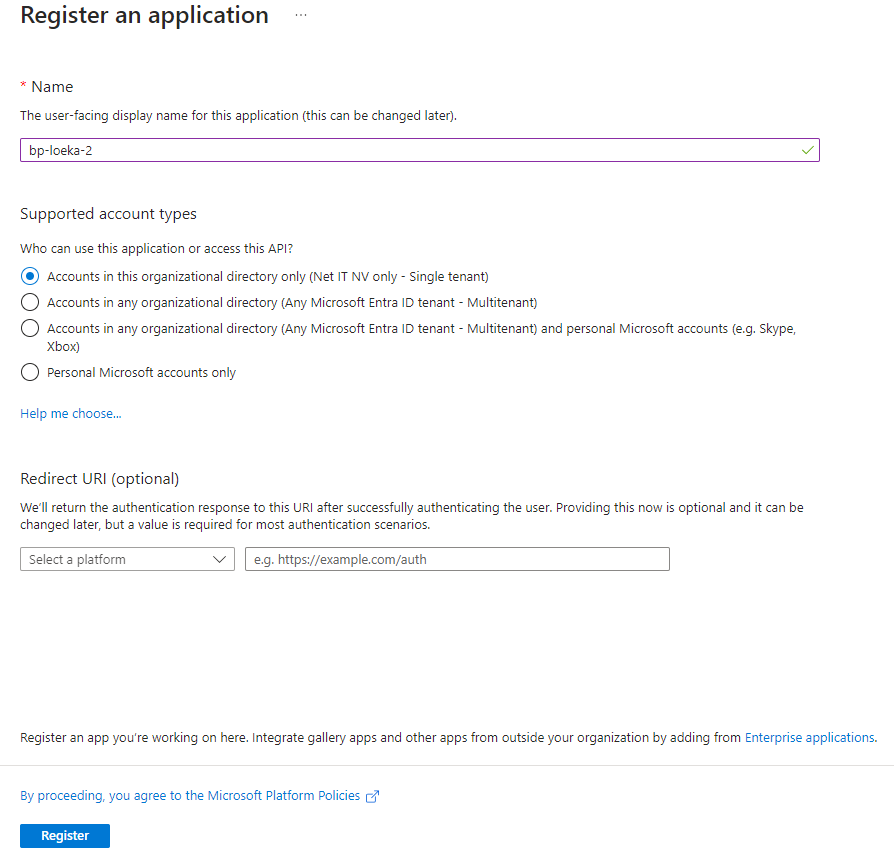
\includegraphics[width=1\textwidth]{./graphics/databricks/connection_2.png}
    \caption{Aanmaken van app registration}
\end{figure}

Door in Microsoft Azure naar ``App registrations'' te navigeren kan er een nieuwe app registration aangemaakt worden.

\begin{figure}[H]
    \centering
    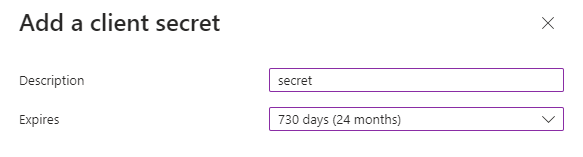
\includegraphics[width=0.9\textwidth]{./graphics/databricks/connection_3.png}
    \caption{Aanmaken client secret}
\end{figure}

Door naar ``Certificates \& secrets'' in de app registration te navigeren kan er een client secret aangemaakt worden. Het is belangrijk om deze client secret op te slaan.

\begin{figure}[H]
    \centering
    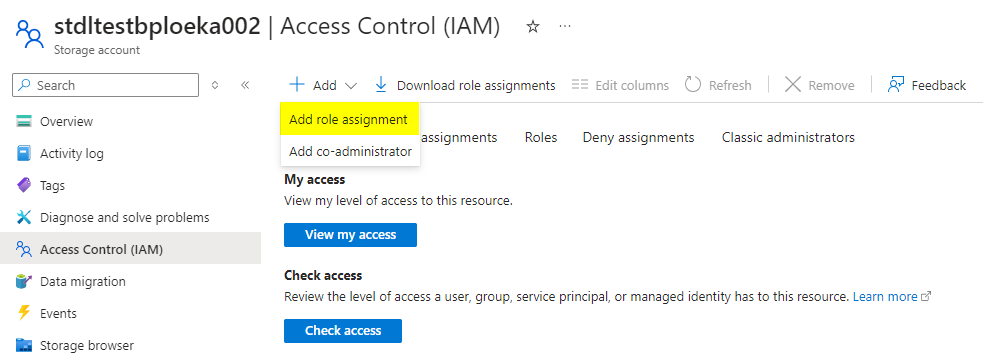
\includegraphics[width=1\textwidth]{./graphics/databricks/connection_4.png}
    \caption{Role assignment toevoegen aan storage account}
\end{figure}

Door naar``Access Control (IAM)'' te navigeren van het storage account waarmee we een connectie willen maken, kunnen we nu een role assignment gaan toevoegen.

\begin{figure}[H]
    \centering
    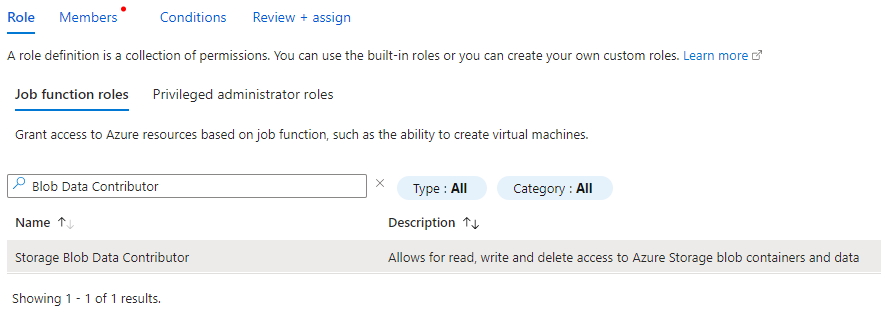
\includegraphics[width=1\textwidth]{./graphics/databricks/connection_5.png}
    \caption{Job function role kiezen voor role assignment}
\end{figure}

Als job function role moet er voor ``Storage Blob Data Contributor'' gekozen worden.

\begin{figure}[H]
    \centering
    \includegraphics[width=1\textwidth]{./graphics/databricks/connection_6.png}
    \caption{Members kiezen voor role assignment}
\end{figure}

Bij ``Members'' kiezen we voor de service principal die we net hebben aangemaakt. Dit zorgt er voor dat de app registration die we net hebben aangemaakt toegang heeft tot het data lake.

\begin{figure}[H]
    \centering
    \includegraphics[width=1\textwidth]{./graphics/databricks/connection_8.png}
    \caption{Aanmaken van key vault}
\end{figure}

Doordat we de client secret die we net hebben aangemaakt niet in onze databricks code willen zetten zal er een key vault aangemaakt worden. Dit kan door in Microsoft Azure naar ``Key vaults'' te navigeren. Bij het aanmaken van een key vault moet er een subscription en resource group gekozen worden. Er kan een nieuwe resource group aangemaakt worden of een reeds bestaande gekozen worden. Daarnaast moet er een naam, gewenste regio en pricing tier gekozen worden.

\begin{figure}[H]
    \centering
    \includegraphics[width=1\textwidth]{./graphics/databricks/connection_9.png}
    \caption{Permission model van key vault}
\end{figure}

Onder ``Access configuration'' wordt er gekozen voor ``Vault access policy'' als permission model.

\begin{figure}[H]
    \centering
    \includegraphics[width=1\textwidth]{./graphics/databricks/connection_10.png}
    \caption{Networking configuratie van key vault}
\end{figure}

Er kan gekozen worden om enkel geselecteerde networks public access te geven of om public access uit te schakelen. Belangrijk is dat ``Allow trusted Microsoft services to bypass this firewall'' aangevinkt staat.

\begin{figure}[H]
    \centering
    \includegraphics[width=1\textwidth]{./graphics/databricks/connection_12.png}
    \caption{Toevoegen van een secret in key vault}
\end{figure}

Door naar ``Secrets'' te navigeren in de key vault kan het client secret toegevoegd worden.

\begin{figure}[H]
    \centering
    \includegraphics[width=1\textwidth]{./graphics/databricks/connection_13.png}
    \caption{Opzoeken van properties van key vault}
\end{figure}

Door naar ``Properties'' te navigeren kunnen we nu ``Vault URI'' en ``Resource ID'' terugvinden. Deze zijn belangrijk voor de volgende stap.

\begin{figure}[H]
    \centering
    \includegraphics[width=0.9\textwidth]{./graphics/databricks/connection_14.png}
    \caption{Aanmaken van secret scope in databricks}
\end{figure}

Door naar ``https://<databricks-instance>\#secrets/createScope'' te navigeren kunnen we nu een secret scope aanmaken in databricks. Hiervoor hebben we ``Vault URI'' en ``Resource ID'' nodig uit de vorige stap.

\begin{minted}{python}
app_key = dbutils.secrets.get(scope = "KeyVault", key = "AppKey")
\end{minted}

We kunnen nu in onze notebooks met bovenstaande code secrets zoals bijvoorbeeld ``AppKey'' ophalen uit key vault.

%\begin{center}
%    \includegraphics[width=0.9\textwidth]{./graphics/databricks/connection_16.png}
%    \footnote{Configuratie van `spark-cdm-connector`}
%\end{center}


\begin{minted}{python}
storage_account = "<storage-account>"
app_id = "<application-id>"
app_key = dbutils.secrets.get(scope = "KeyVault", key = "AppKey")
tenant_id = "<directory-id>"
\end{minted}


Om een connectie te kunnen maken met data lake hebben we ``storage\_account'', ``app\_id'', ``app\_key'' en ``tenant\_id'' nodig. Dit kunnen we doen door het volgende te vervangen:

\begin{itemize}
    \item ``<storage-account>'' met de naam van het Azure storage account
    \item ``<application-id>'' met het Application (client) ID voor de Microsoft Entra ID application
    \item ``<directory-id>'' met het Directory (tenant) ID voor de Microsoft Entra ID application
\end{itemize}

% TODO Meer uitleg geven hierboven over in literatuurstudie?

%\begin{center}
%    \includegraphics[width=0.9\textwidth]{./graphics/databricks/connection_17.png}
%    \footnote{Configuratie van `spark-cdm-connector`}
%\end{center}

\begin{minted}{python}
df = spark.read.format("com.microsoft.cdm") \
    .option("appId", app_id) \
    .option("appKey", app_key) \
    .option("tenantId", tenant_id) \
    .option("storage", f"{storage_account}.dfs.core.windows.net") \
    .option("manifestPath", "sourcedata/model.json") \
    .option("mode", "permissive")
\end{minted}

We kunnen nu gebruik maken van ``spark-cdm-connector'' door ``com.microsoft.cdm'' mee te geven. Het is belangrijk dat ``mode'' op ``permissive'' staat, dit zorgt er voor dat er ``NULL'' values assigned worden wanneer een CSV rij minder aantal kolommen heeft dan het entity schema.

%\begin{center}
%    \includegraphics[width=0.9\textwidth]{./graphics/databricks/connection_18.png}
%    \footnote{Laden van de nodige entiteiten in databricks}
%\end{center}

\begin{minted}{python}
spr = df.option("entity", "new_syndicalpremiumrequest") \
    .load()
\end{minted}

Met bovenstaande code kan een entiteit ingeladen worden in een variabele. Dit zal dus ook gebeuren met alle entiteiten die we hebben.

%\begin{center}
%    \includegraphics[width=0.9\textwidth]{./graphics/databricks/connection_19.png}
%    \footnote{Selecteren van kolommen en aanmaken van temporary views in databricks}
%\end{center}

\begin{minted}{python}
spr \
    .select("Id", "new_personid", "new_bankaccountid", "new_scannedrequestcode", "new_isdeclarationonhonour", "new_requesttypeid", "new_formnumber", "new_treatmentstate", "new_feedback", "new_reasonforcontrol", "new_yearid", "createdon", "new_idadm", "new_contributionamount", "new_premiumamount", "new_paymentdate", "new_remarkgroupfinal", "new_groupid") \
    .createOrReplaceTempView("new_syndicalpremiumrequest")
\end{minted}

Voor elke entiteit die we hebben ingeladen in een variabele zullen we nu de nodige kolommen gaan selecteren. Hierna kan er een temporary view aangemaakt worden voor de entiteiten. Daardoor kunnen we later queries gaan uitvoeren in SQL om zo transformaties uit te voeren.

\subsection{Mogelijkheid tot debuggen}

\begin{figure}[H]
    \centering
    \includegraphics[width=1\textwidth]{./graphics/databricks/debug.png}
    \caption{Debuggen in Azure Databricks}
\end{figure}

In Azure Databricks kan er telkens geprint worden welke output bepaalde code geeft. Bij SQL statements zal dit bijvoorbeeld resulteren in een tabel. Op deze tabel kan er gefilterd worden of kunnen zelfs visualisaties gemaakt worden. Het maximum aantal resultaten dat hier bij getoond zal worden is 10.000 rijen of 2MB. In Databricks Runetime 12.2 LTS kan dit maximum verhoogd worden. Daarnaast is er ook een interactieve debugger in ``Public Preview''. Hier gaan we verder niet op ingaan aangezien deze Databricks Runtime version 13.3 LTS of hoger nodig heeft en wij een oudere versie gebruiken om Common Data Model te gebruiken.

\subsection{Belangrijkste transformaties}

\subsubsection{Determinatie van welke groepen de premie in hun bestand krijgen}

\begin{minted}[highlightlines={4, 5, 6, 56}]{sql}
CREATE
OR REPLACE TEMPORARY VIEW spr_stage_1 AS
SELECT 
    YEAR(spr.createdon) EntryYear, 
    YEAR(GETDATE()) CalendarYear, 
    CAST(ny.new_year AS INTEGER) RefYear, 
    IF(spr.new_scannedrequestcode == 552010000, IF(spr.new_isdeclarationonhonour, "DOH", "FORM"), IF(spr.new_scannedrequestcode == 552010001, "QR", "UNKNOWN")) Type,
    
    IF(spr.new_requesttypeid == "d026f6f9-fc82-ea11-a811-000d3a2d0171", CONCAT(SUBSTRING(new_formnumber, 1, 4), "-", SUBSTRING(new_formnumber, 5, 6), "-", SUBSTRING(new_formnumber, 11, 20)), spr.new_formnumber) Form,
    
    IF(rpr.new_treatmentstate == 552010004,
        CASE
            WHEN spr.new_treatmentstate == 552010000 THEN "1"
            WHEN spr.new_treatmentstate == 552010001 THEN "10"
            WHEN spr.new_treatmentstate == 552010002 THEN "1"
            WHEN spr.new_treatmentstate == 552010003 THEN "10"
            WHEN spr.new_treatmentstate == 552010004 THEN "5"
            WHEN spr.new_treatmentstate == 552010005 THEN "11"
            WHEN spr.new_treatmentstate == 552010006 THEN "1"
            WHEN spr.new_treatmentstate == 552010007 THEN "10"
            WHEN spr.new_treatmentstate == 552010008 THEN "8"
            ELSE ""
        END,
        CASE
            WHEN spr.new_treatmentstate == 552010000 THEN "1"
            WHEN spr.new_treatmentstate == 552010001 THEN "2"
            WHEN spr.new_treatmentstate == 552010002 THEN "1"
            WHEN spr.new_treatmentstate == 552010003 THEN "2"
            WHEN spr.new_treatmentstate == 552010004 THEN "5"
            WHEN spr.new_treatmentstate == 552010005 THEN "11"
            WHEN spr.new_treatmentstate == 552010006 THEN "1"
            WHEN spr.new_treatmentstate == 552010007 THEN "2"
            WHEN spr.new_treatmentstate == 552010008 THEN "8"
            ELSE ""
        END
    ) Status,
    IF(spr.new_feedback, "FEEDBACK", spr.new_reasonforcontrol) AvalonRemark,
    
    spr.new_personid,
    spr.new_idadm,
    spr.new_yearid,
    spr.id,
    spr.createdon,
    spr.new_contributionamount,
    spr.new_premiumamount,
    spr.new_paymentdate,
    ba.new_bankaccount,
    spr.new_remarkgroupfinal,
    p.new_firstname,
    p.new_lastname,
    p.new_dateofbirth
FROM new_syndicalpremiumrequest spr
LEFT JOIN new_person p ON spr.new_personid = p.new_personid
LEFT JOIN new_bankaccount ba ON spr.new_bankaccountid = ba.new_bankaccountid
LEFT JOIN related_premium_requests rpr ON spr.Id = rpr.new_syndicalpremiumrequestid
LEFT JOIN new_year ny ON spr.new_yearid = ny.new_yearid;
\end{minted}

De tabel ``new\_year'' wordt opnieuw gejoind op de tabel ``new\_syndicalpremiumrequest'' met behulp van de kolom ``new\_yearid''. Daarnaast worden ook hier de drie kolommen ``EntryYear'', ``CalendarYear'' en ``RefYear'' berekent. Deze worden op dezelfde manier berekent als bij de transformatie in Azure Data Factory.


\begin{minted}{sql}
CREATE
OR REPLACE TEMPORARY VIEW spr_stage_2 AS
SELECT 
    explode(array(nm.new_groupid, noy.new_groupid)) new_groupid,
    spr.*,
    nm.new_groupprefix new_groupprefix
FROM spr_stage_1 spr
LEFT JOIN new_membership_stage_1 nm 
    ON (spr.CalendarYear = nm.new_year OR spr.EntryYear = nm.new_year OR RefYear == nm.new_year) AND spr.new_personid == nm.new_personid 
LEFT JOIN new_organizationyear_stage_1 noy 
    ON spr.new_idadm == noy.new_idadmaux AND spr.new_yearid == noy.new_yearid;
\end{minted}

De tabellen ``new\_membership'' en ``new\_organizationyear'' worden gejoind op de tabel ``new\_syndicalpremiumrequest'' om de groepen te gaan bepalen. Zoals te zien in de code snippet hierboven noemen deze tabellen ``new\_membership\_stage\_1'' en ``new\_organizationyear\_stage\_1''. Dit komt doordat er reeds andere transformaties zijn geweest.

Bij de tabel ``new\_membership'' wordt er, net zoals in Azure Data Factory, gekeken of ``CalendarYear'', ``EntryYear'' of ``RefYear'' overeenkomt met het jaartal van de membership. Daarnaast wordt er ook gekeken of personid overeen komt. 

Bij de tabel ``new\_organizationyear'' wordt er gejoind met behulp van IDADM en het id van het referentiejaar.

\begin{figure}[H]%
    \centering
    \begin{tabularx}{0.9\textwidth}{ |X|X|X| }
        \hline
        \textbf{spr.Id} & \textbf{nm.new\_groupid} & \textbf{noy.new\_groupid} \\
        \hline 
        101e4523-7c60-45ff-a928-087ca139d8f5  & 2ad31fb8-5117-4627-a2a3-a5fdbee5b9ae & null  \\
        \hline
        f5ac28c0-6b80-412a-b0e6-f9a82feff9a1 & f1015dd0-3096-478d-ae12-4226c101dd54 & a2974e74-be93-4326-9d18-f4bb2abc0842 \\
        \hline
    \end{tabularx}
    
    \Bigg\downarrow
    
    \begin{tabularx}{0.9\textwidth}{ |X|X| }
        \hline
        \textbf{spr.Id} & \textbf{new\_groupid} \\
        \hline 
        101e4523-7c60-45ff-a928-087ca139d8f5  & 2ad31fb8-5117-4627-a2a3-a5fdbee5b9ae  \\
        \hline
        101e4523-7c60-45ff-a928-087ca139d8f5  & null  \\
        \hline
        f5ac28c0-6b80-412a-b0e6-f9a82feff9a1 & f1015dd0-3096-478d-ae12-4226c101dd54 \\
        \hline
        f5ac28c0-6b80-412a-b0e6-f9a82feff9a1 & a2974e74-be93-4326-9d18-f4bb2abc0842 \\
        \hline
    \end{tabularx}
    \caption{Voorbeeld van hoe de functie explode werkt.}
%    TODO klopt deze caption in zogezegde picture?
\end{figure}

Deze twee joins resulteren in twee nieuwe kolommen ``nm.new\_groupid'' en ``noy.new\_groupid''. Met behulp van de ``explode'' functie zorgen we er voor dat deze twee kolommen één kolom zullen worden. Één rij zal dan bijvoorbeeld twee rijen worden. Deze twee rijen zijn dan volledig hetzelfde met het verschil dat de kolom ``new\_groupid'' voor de eerste rij de waarde van ``nm.new\_groupid'' heeft en voor de tweede rij de waarde van ``noy.new\_groupid''.


\begin{minted}{sql}
CREATE 
OR REPLACE TEMPORARY VIEW spr_stage_3 AS 
SELECT 
    FIRST(id) id, 
    FIRST(new_groupid) new_groupid, 
    FIRST(new_personid) new_personid,
    FIRST(CalendarYear) CalendarYear,
    FIRST(EntryYear) EntryYear,
    FIRST(RefYear) RefYear,
    FIRST(new_groupprefix) new_groupprefix,
    FIRST(createdon) createdon,
    FIRST(new_contributionamount) new_contributionamount,
    FIRST(new_premiumamount) new_premiumamount,
    FIRST(new_paymentdate) new_paymentdate,
    FIRST(new_bankaccount) new_bankaccount,
    FIRST(new_remarkgroupfinal) new_remarkgroupfinal,
    FIRST(AvalonRemark) AvalonRemark,
    FIRST(new_firstname) new_firstname,
    FIRST(new_lastname) new_lastname,
    FIRST(new_dateofbirth) new_dateofbirth,
    FIRST(Type) Type,
    FIRST(Form) Form,
    FIRST(Status) Status,
    FIRST(new_idadm) new_idadm
FROM spr_stage_2 
WHERE id IS NOT NULL AND new_groupid IS NOT NULL AND RefYear IS NOT NULL
GROUP BY (id, new_groupid, RefYear);
\end{minted}

Ten slotte wordt er een ``GROUP BY'' clause gebruikt om er voor te zorgen dat een premie niet twee keer naar dezelfde groep voor dat referentiejaar wordt gestuurd. Daarnaast wordt er ook gefilterd zodat er geen premies zijn zonder id, groupid of referentiejaar. Met behulp van de ``FIRST'' aggregrate function selecteren we steeds de eerste waarde voor de nodige kolommen. We hebben nu een tabel met alle premies waarvan we weten naar welke groep voor welk referentiejaar ze gestuurd moeten worden.

\subsubsection{Bepalen van de kolom ``Gr'' voor een premie}

\begin{minted}[highlightlines={4}]{sql}
CREATE
OR REPLACE TEMPORARY VIEW nm_grouped_by AS
SELECT 
    FIRST(new_groupprefix, TRUE) new_groupprefix, 
    FIRST(new_personid) new_personid, 
    FIRST(new_year) new_year 
FROM new_membership_stage_1
WHERE new_groupprefix IS NOT NULL 
GROUP BY (new_personid, new_year);

CREATE 
OR REPLACE TEMPORARY VIEW spr_stage_4 AS 
SELECT
    spr.*,
    CASE
        WHEN spr.new_groupprefix IS NOT NULL THEN spr.new_groupprefix
        WHEN nmCalendar.new_groupprefix IS NOT NULL THEN nmCalendar.new_groupprefix
        WHEN nmEntry.new_groupprefix IS NOT NULL THEN nmEntry.new_groupprefix
        WHEN nmRef.new_groupprefix IS NOT NULL THEN nmRef.new_groupprefix
        ELSE NULL
    END Gr
FROM spr_stage_3 spr
LEFT JOIN nm_grouped_by nmCalendar ON spr.new_personid = nmCalendar.new_personid AND spr.CalendarYear = nmCalendar.new_year
LEFT JOIN nm_grouped_by nmEntry ON spr.new_personid = nmEntry.new_personid AND spr.EntryYear = nmEntry.new_year
LEFT JOIN nm_grouped_by nmRef ON spr.new_personid = nmRef.new_personid AND spr.RefYear = nmRef.new_year;
\end{minted}

Voor het bepalen van de kolom ``Gr'' in databricks wordt er eerst een temporary view ``nm\_grouped\_by'' aangemaakt waarbij er gegroepeerd wordt op ``new\_personid'' en ``new\_year''. Dit zal er voor zorgen dat de joins die we uitvoeren zullen resulteren in één enkele match (of geen). De tweede parameter in de functie ``FIRST'' (aangeduid in code snippet) zorgt er voor dat ``NULL'' values genegeerd worden. De eeste waarde die niet ``NULL'' is voor ``new\_groupprefix'' zal dus geselecteerd worden.

De temporary view die we hebben aangemaakt wordt nu drie keer gejoind op de tabel ``spr\_stage\_3'' aan de hand van ``new\_personid'' en ``CalendarYear'', ``EntryYear'' of ``RefYear''. ``Gr'' zal bepaald worden door eerst te kijken of ``spr.new\_groupprefix'' niet ``NULL'' is, wanneer deze wel ``NULL'' is zal er gekeken worden naar ``nmCalendar.new\_groupprefix'', ``nmEntry.new\_groupprefix'' en ten slotte naar ``nmRef.new\_groupprefix''.

\subsubsection{Bepalen van de kolommen ``AntheaNumber'' en ``MembershipNumber'' voor een premie}

\begin{minted}{sql}
%sql
CREATE
OR REPLACE TEMPORARY VIEW nm_grouped_by_2 AS
SELECT 
    FIRST(new_antheanumber, TRUE) new_antheanumber,
    FIRST(new_newmembershipnumber, TRUE) new_newmembershipnumber,
    FIRST(new_groupid) new_groupid, 
    FIRST(new_year) new_year,
    FIRST(new_personid) new_personid
FROM new_membership_stage_1
WHERE new_antheanumber IS NOT NULL OR new_newmembershipnumber IS NOT NULL
GROUP BY (new_groupid, new_year, new_personid);

CREATE 
OR REPLACE TEMPORARY VIEW spr_stage_5 AS 
SELECT
    spr.*,
    CASE
        WHEN Gr IS NULL THEN NULL
        WHEN nmCalendar.new_antheanumber IS NOT NULL THEN nmCalendar.new_antheanumber
        WHEN nmEntry.new_antheanumber IS NOT NULL THEN nmEntry.new_antheanumber
        WHEN nmRef.new_antheanumber IS NOT NULL THEN nmRef.new_antheanumber
        ELSE NULL
    END AntheaNumber,
    CASE
        WHEN Gr IS NULL THEN NULL
        WHEN nmCalendar.new_newmembershipnumber IS NOT NULL THEN nmCalendar.new_newmembershipnumber
        WHEN nmEntry.new_newmembershipnumber IS NOT NULL THEN nmEntry.new_newmembershipnumber
        WHEN nmRef.new_newmembershipnumber IS NOT NULL THEN nmRef.new_newmembershipnumber
        ELSE NULL
    END MembershipNumber
FROM spr_stage_4 spr
LEFT JOIN nm_grouped_by_2 nmCalendar ON spr.new_groupid = nmCalendar.new_groupid AND spr.CalendarYear = nmCalendar.new_year AND spr.new_personid = nmCalendar.new_personid
LEFT JOIN nm_grouped_by_2 nmEntry ON spr.new_groupid = nmEntry.new_groupid AND spr.EntryYear = nmEntry.new_year AND spr.new_personid = nmEntry.new_personid  
LEFT JOIN nm_grouped_by_2 nmRef ON spr.new_groupid = nmRef.new_groupid AND spr.RefYear = nmRef.new_year AND spr.new_personid = nmRef.new_personid;
\end{minted}

Voor het bepalen van de kolommen ``AntheaNumber'' en ``MembershipNumber'' wordt er eerst een temporary view ``nm\_grouped\_by\_2'' aangemaakt waarbij er gegroepeerd wordt op ``new\_groupid'', ``new\_year'' en ``new\_personid''. Dit zal er voor zorgen dat de joins die uitgevoerd worden resulteren in één enkele match (of geen). De functie ``FIRST'' zorgt er weer voor dat ``NULL'' values genegeerd worden. De aangemaakte temporary view wordt nu drie keer gejoind op de tabel ``spr\_stage\_4'' aan de hand van ``new\_groupid'', ``new\_personid'' en ``CalendarYear'', ``EntryYear'' of ``RefYear''. Wanneer de kolom ``Gr'', ``NULL'' is, zal ``AntheaNumber'' en ``MembershipNumber'' ook ``NULL zijn. Wanneer dit niet zo is wordt eerst gekeken of de waarde van de join aan de hand van ``CalendarYear'' niet ``NULL'' is. Wanneer dit wel ``NULL'' is zal er vervolgens gekeken worden naar de join aan de hand van ``EntryYear'' en vervolgens naar de join aan de hand van ``RefYear''.

\subsection{Schrijven van data naar Azure Data Lake}

\begin{minted}{sql}
SELECT 
    RefYear, 
    new_groupid `Group`,
    Gr, 
    id Id, 
    createdon EntryDate,
    Type,
    Form,
    new_contributionamount Contribution,
    new_premiumamount Prem,
    Status,
    new_paymentdate PayDate,
    new_bankaccount Account,
    new_remarkgroupfinal Remark,
    AvalonRemark,
    new_lastname `Name`,
    new_firstname FirstName,
    new_dateofbirth BirthDay,
    CalendarYear,
    EntryYear,
    AntheaNumber,
    MembershipNumber,
    new_idadm IdAdm,
    new_groupprefix IDADM_Gr
FROM spr_stage_5;
\end{minted}

De laatste SQL statement die de data bevat die naar Azure Data Lake geschreven moet worden wordt niet in temporary view gestoken. Databricks zal de output van deze SQL statement automatisch in een PySpark data frame genaamd ``\_sqldf'' steken.

\begin{minted}{python}
spark.conf.set(f"fs.azure.account.auth.type.{storage_account}.dfs.core.windows.net", "OAuth")
spark.conf.set(f"fs.azure.account.oauth.provider.type.{storage_account}.dfs.core.windows.net", "org.apache.hadoop.fs.azurebfs.oauth2.ClientCredsTokenProvider")
spark.conf.set(f"fs.azure.account.oauth2.client.id.{storage_account}.dfs.core.windows.net", app_id)
spark.conf.set(f"fs.azure.account.oauth2.client.secret.{storage_account}.dfs.core.windows.net", app_key)
spark.conf.set(f"fs.azure.account.oauth2.client.endpoint.{storage_account}.dfs.core.windows.net", f"https://login.microsoftonline.com/{tenant_id}/oauth2/token")

_sqldf.coalesce(1).write.option("header", "true").mode("overwrite").csv(f"abfss://target@{storage_account}.dfs.core.windows.net/databricks")
\end{minted}

Met behulp van ``\_sqldf'' in Python en de variabelen die we eerder hebben geïnitialiseerd, zoals te zien in sectie~\ref{sec:ophalen}, wordt er terug naar Azure Data Lake geschreven. Hierbij wordt er gebruik gemaakt van ``.coalesce(1)'' om aan te geven dat er naar slechts één CSV bestand geschreven moet worden.

\section{Validatie van output}

Het exportbestand voor zowel Azure Data Factory als Azure Databricks kan in Microsoft Power BI ingeladen worden om te vergelijken of de data overeenkomt. 

\begin{minted}{text}
= Table.RemoveMatchingRows(#"ADF", Table.ToRecords(#"DATABRICKS"), { "Id", "Group", "RefYear" })
\end{minted}

Bovenstaande Power Query gaat een tabel aanmaken met rijen die geen matches hebben voor de kolom ``Id'', ``Group'' en ``RefYear''. Wanneer dit dus een lege tabel geeft betekent dit dus dat beide exportbestanden even veel rijen hebben waarbij voor elke rij van Azure Data Factory een rij is in het bestand van Azure Databricks waarbij deze overeen komen. Er kunnen ook andere kolommen toegevoegd worden om deze te gaan valideren of het laatste argument kan weg gelaten worden om de volledige CSV bestanden te gaan valideren.